\documentclass[12pt,a4paper]{report}
\usepackage[utf8]{vietnam}
\usepackage[english]{babel} 
\usepackage[margin=2cm]{geometry}
\usepackage{setspace} 
\usepackage{hyperref}
\usepackage{xcolor}
\usepackage{titlesec}
\usepackage{float}
\usepackage{graphicx}

% \usepackage{amsmath}
% \usepackage{longtable}
% \usepackage{array}
% \usepackage{listings}
% \usepackage{multirow}

\titleformat{\chapter}[hang]{\bfseries\Huge}
  {Chapter \thechapter:}{1em}{}

\hypersetup{
    colorlinks=true,        % Bật màu cho liên kết
    linkcolor=blue,         % Màu cho các liên kết nội bộ (nếu có)
    urlcolor=blue,          % Màu cho các liên kết URL
    filecolor=magenta,      % Màu cho liên kết đến file (nếu có)
    pdftitle={My PDF},      % Tiêu đề của PDF (tùy chọn)
    pdfauthor={Author},     % Tác giả của PDF (tùy chọn)
}

\begin{document}
\setstretch{1.5}  % Giảm khoảng cách giữa các dòng (1.0 là bình thường, giảm xuống < 1.0 sẽ làm chúng gần nhau hơn)

% Trang bìa
\begin{titlepage}
   \begin{center}
      \textbf{\Large POSTS AND TELECOMMUNICATIONS INSTITUTE OF TECHNOLOGY}
   \end{center}
    
   \begin{center}
      \textbf{\Large FACULTY OF INFORMATION TECHNOLOGY I}
   \end{center}
    
   \begin{center}
      \textbf{\Large PYTHON PROGRAMMING COURSE}
   \end{center}
    
   \vspace{1cm}  % Giảm khoảng cách để các phần không quá cách xa nhau
   \begin{center}
      
\includegraphics[width=2in, height=2.5in]{media/image7.png}
   \end{center}
    
   \vspace{1.5cm}  % Điều chỉnh khoảng cách để phần văn bản và bảng cân đối
   \begin{center}
      \textbf{\LARGE ASSIGNMENT REPORT}
   \end{center}
    
   \vspace{1cm}  % Điều chỉnh khoảng cách cho phần bảng
   \begin{center}
      \begin{tabular}{p{4cm} l}
          \textbf{Lecturer}     & : KIM NGOC BACH \\[0.3cm]  % Thêm khoảng cách nhỏ giữa các dòng
          \textbf{Student}      & : DAO VAN KHANG \\[0.3cm] 
          \textbf{Student ID}   & : B23DCVT218 \\[0.3cm]
          \textbf{Class}        & : D23CQCE04-B \\[0.3cm]
          \textbf{Group}        & : 04 \\[0.3cm]
      \end{tabular}
  \end{center}  

   \vfill  % Giữ khoảng cách phía dưới cân đối
   \begin{center}
      \textbf{\large Ha Noi -- 2025}
   \end{center}
\end{titlepage}

% Tóm tắt
\setlength{\parindent}{0em}  % Bỏ thụt lề
\setlength{\parskip}{1em}    % Khoảng cách giữa các đoạn

% Chèn phần Summary trước Table of Contents
\cleardoublepage  % Bắt đầu trang mới
\phantomsection  % Đảm bảo tính tương thích với hyperref
\addcontentsline{toc}{chapter}{Summary}  % Thêm phần Summary vào mục lục
\chapter*{Summary}  % Không đánh số cho phần này
This report documents the implementation of Python Programming Assignment 1 for the 2024--2025 academic year. The objective of the assignment is to apply practical Python programming skills to the domain of football analytics, using real-world data from the English Premier League.

The task is divided into four parts. In the first part, a Python program is developed to collect statistical data for all players who have played more than 90 minutes during the 2024--2025 season. The data is sourced from the website \href{https://fbref.com}{fbref.com} and includes a wide range of metrics related to performance, goalkeeping, passing, shooting, possession, and more. The collected data is saved to a file named \texttt{results.csv}, with players sorted alphabetically by first name and unavailable statistics marked as "N/a".

The second part involves statistical analysis of the collected dataset. It includes identifying the top three and bottom three players for each statistic, and computing the median, mean, and standard deviation values per attribute across all players and per team. The results are saved to \texttt{top\_3.txt} and \texttt{results2.csv}. Additionally, histograms are plotted to visualize the distribution of each statistic, and a comparative analysis is conducted to determine the best-performing team.

The third part applies machine learning techniques to classify players based on their statistical profiles. The K-means clustering algorithm is used, and Principal Component Analysis (PCA) is employed to reduce the data to two dimensions for visualization.

In the final part, transfer values for players with more than 900 minutes of play are collected from \href{https://footballtransfers.com}{FootballTransfers.com}. A method for estimating player value is proposed, an explanation of feature selection and model choice.

\setstretch{1.2}  % Giảm khoảng cách giữa các dòng (1.0 là bình thường, giảm xuống < 1.0 sẽ làm chúng gần nhau hơn)

% Mục lục
\tableofcontents

% Danh mục hình ảnh (List of Figures)
\cleardoublepage  % Start on a new right-hand page
\phantomsection  % For hyperref compatibility
\addcontentsline{toc}{chapter}{\listfigurename}  % Add to TOC
\listoffigures

\setstretch{1.5}  % Giảm khoảng cách giữa các dòng (1.0 là bình thường, giảm xuống < 1.0 sẽ làm chúng gần nhau hơn)

% Phần I
\chapter{Data Collection}
\section{Objective}
The goal of this section was to write a Python script to collect statistical data for all football players in the English Premier League (EPL) 2024--2025 season who have played more than 90 minutes from \href{https://fbref.com/en/}{FBref.com}. The dataset must be structured, cleaned, and exported into a CSV file named \texttt{results.csv}.

\section{Tools and Libraries Used}
   \texttt{requests:} for sending HTTP requests to the data source.
   
   \texttt{BeautifulSoup:} for parsing and scraping HTML content.
   
   \texttt{pandas:} to manipulate tabular data, merge multiple datasets, and export the final DataFrame to a CSV file.
   
   \texttt{time:} to delay requests between URL calls to prevent being rate-limited.

\section{Methodology}
\subsection{URL Management}
All URLs were stored in a dictionary called \texttt{url\_dict}, each pointing to a different stat category.

\subsection{Table Extraction}
A function \texttt{get\_frame\_from\_url()} was implemented to:
\begin{itemize}
    \item Download HTML content from each stats page.
    \item Clean HTML comments that often wrap table content on FBref.
    \item Parse the \texttt{<table>} with \texttt{class min\_width sortable stats\_table...}
    \item Extract column headers with group prefixes for clarity.
    \item Convert each row to a structured format and store it in a pd.DataFrame.
\end{itemize}

\subsection{Data Integration}
All dataframes were merged using the shared keys: \texttt{Player, Nation, Pos, and Squad.} 

Duplicate entries were removed using these keys.

\subsection{Filtering and Cleaning}
   Players who played fewer than 90 minutes were removed \texttt{(stats\_Playing Time\_Min > 90).}
   
   Nationalities were cleaned to be in uppercase abbreviation form \texttt{("England" → "ENG").}
   
   Final data was sorted alphabetically by player name.

\subsection{Output}
   Relevant columns were selected using a mapping dictionary \texttt{(column\_mapping).}
   
   Empty or missing values were replaced with \texttt{"N/a".}
   
   The final structured DataFrame was saved to \texttt{result.csv.}

\section{Result}
The final dataset was saved to \texttt{result.csv} and contains full statistics for all EPL players with more than 90 minutes played. The data is clean, structured, and ready for subsequent analysis (Parts II--IV of the assignment).

\begin{figure}[H]
    \centering
    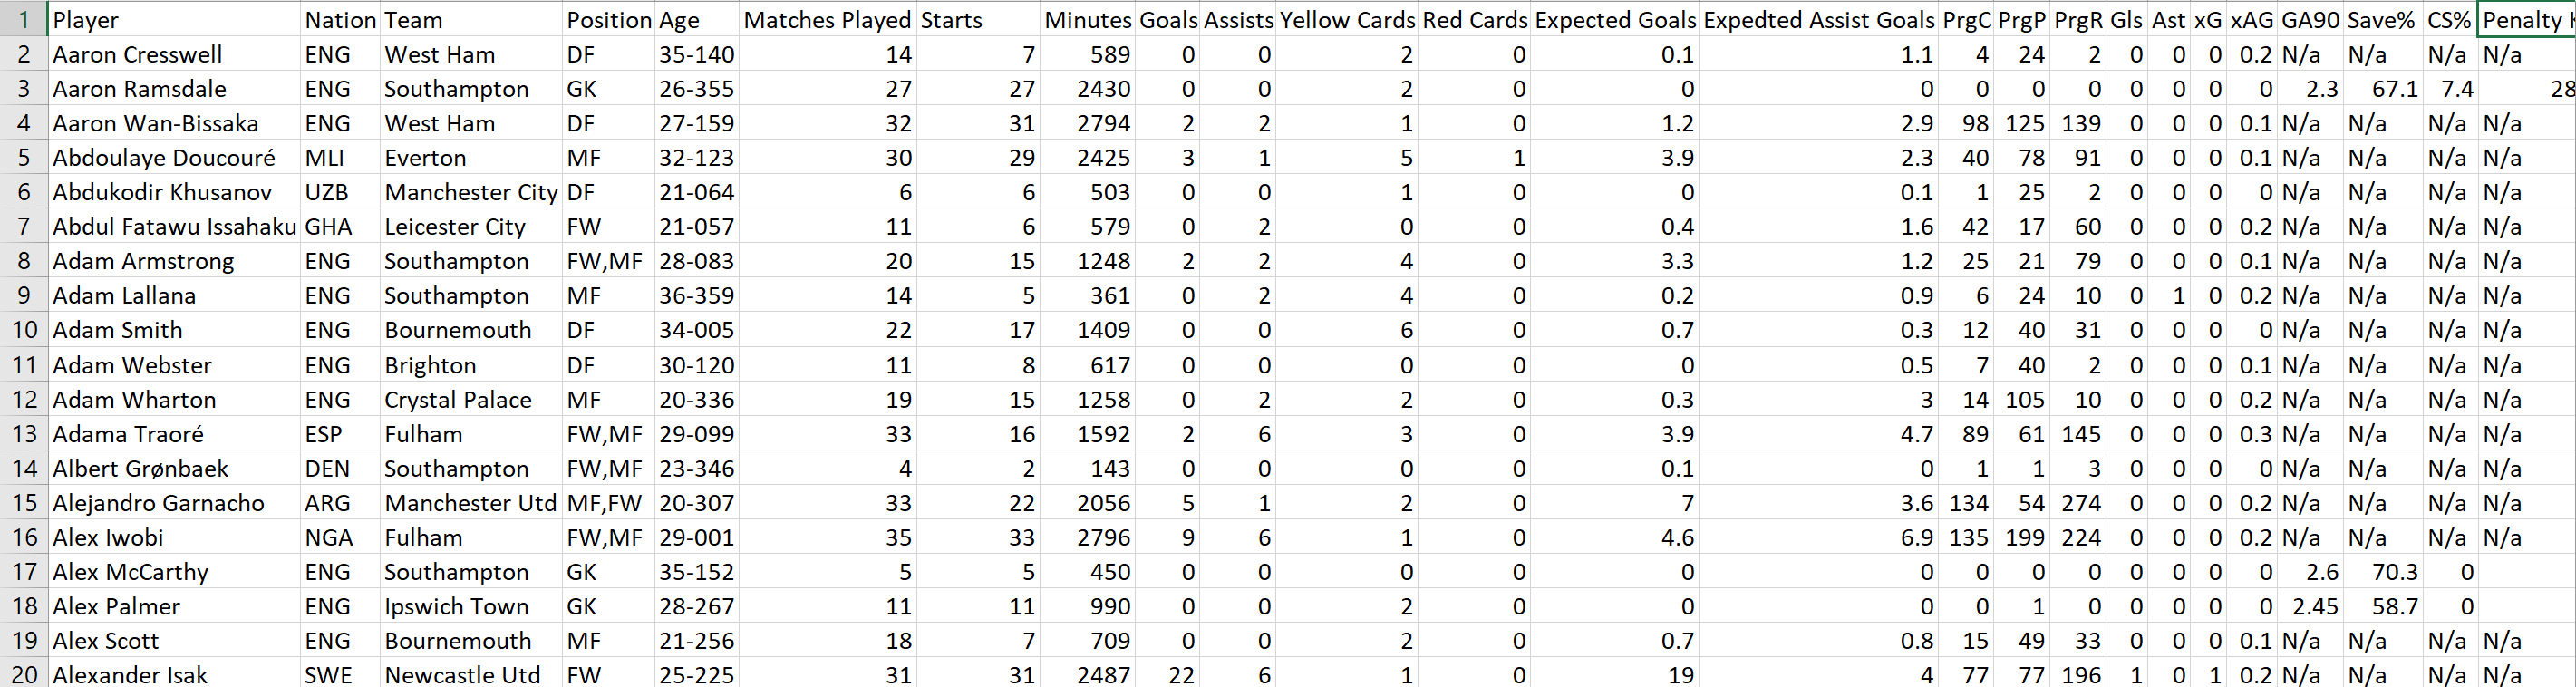
\includegraphics[width=6.5in,height=1.75in]{media/image10.png}
    \caption{Example of collected data}
\end{figure}

% Phần II
\chapter{Statistical Analysis \& Visualization}
\section{Objective}
This part of the assignment focuses on analyzing the football player data collected previously by:
\begin{itemize}
    \item Identifying top-performing players.
    \item Summarizing statistical distributions across the league and by team.
    \item Visualizing data using histograms.
    \item Determining the best-performing team in the 2024--2025 Premier League season.
\end{itemize}

\section{Tools and Libraries Used}
   \texttt{pandas:} for numerical and statistical computation.

   \texttt{matplotlib:} for generating histograms and saving them into PDF.
   
   \texttt{tabulate:} for formatting output text for top 3 rankings.

\section{Methodology}
\subsection{Top 3 and Bottom 3 Players by Statistic}
A function \texttt{identify\_the\_top\_3\_each\_statistic()} was developed to:
\begin{itemize}
    \item Identify and export top 3 and bottom 3 players for each statistic.
    \item Write results to \texttt{top\_3.txt} using a formatted table for clarity.
\end{itemize}

\begin{figure}[H]
    \centering
    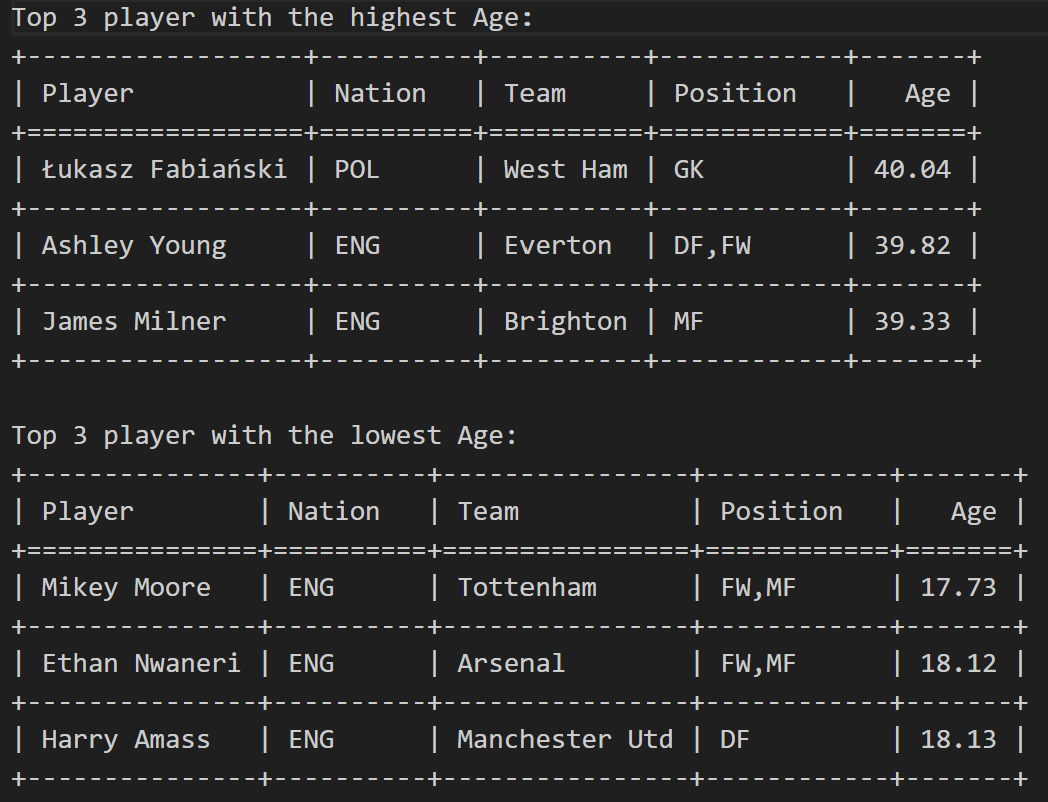
\includegraphics[width=6.5in,height=4.5in]{media/image14.png}
    \caption{Top 3 players example}
\end{figure}

\subsection{Summary Statistics}
In \texttt{find\_median\_mean\_and\_standard\_each\_statistic():}
\begin{itemize}
    \item \textbf{Median}, \textbf{Mean}, and \textbf{Standard Deviation} were calculated for:
    \begin{itemize}
        \item All players in the league.
        \item Each individual team.
    \end{itemize}
    \item The final results were exported to \texttt{result2.csv.}
\end{itemize}

\begin{figure}[H]
    \centering
    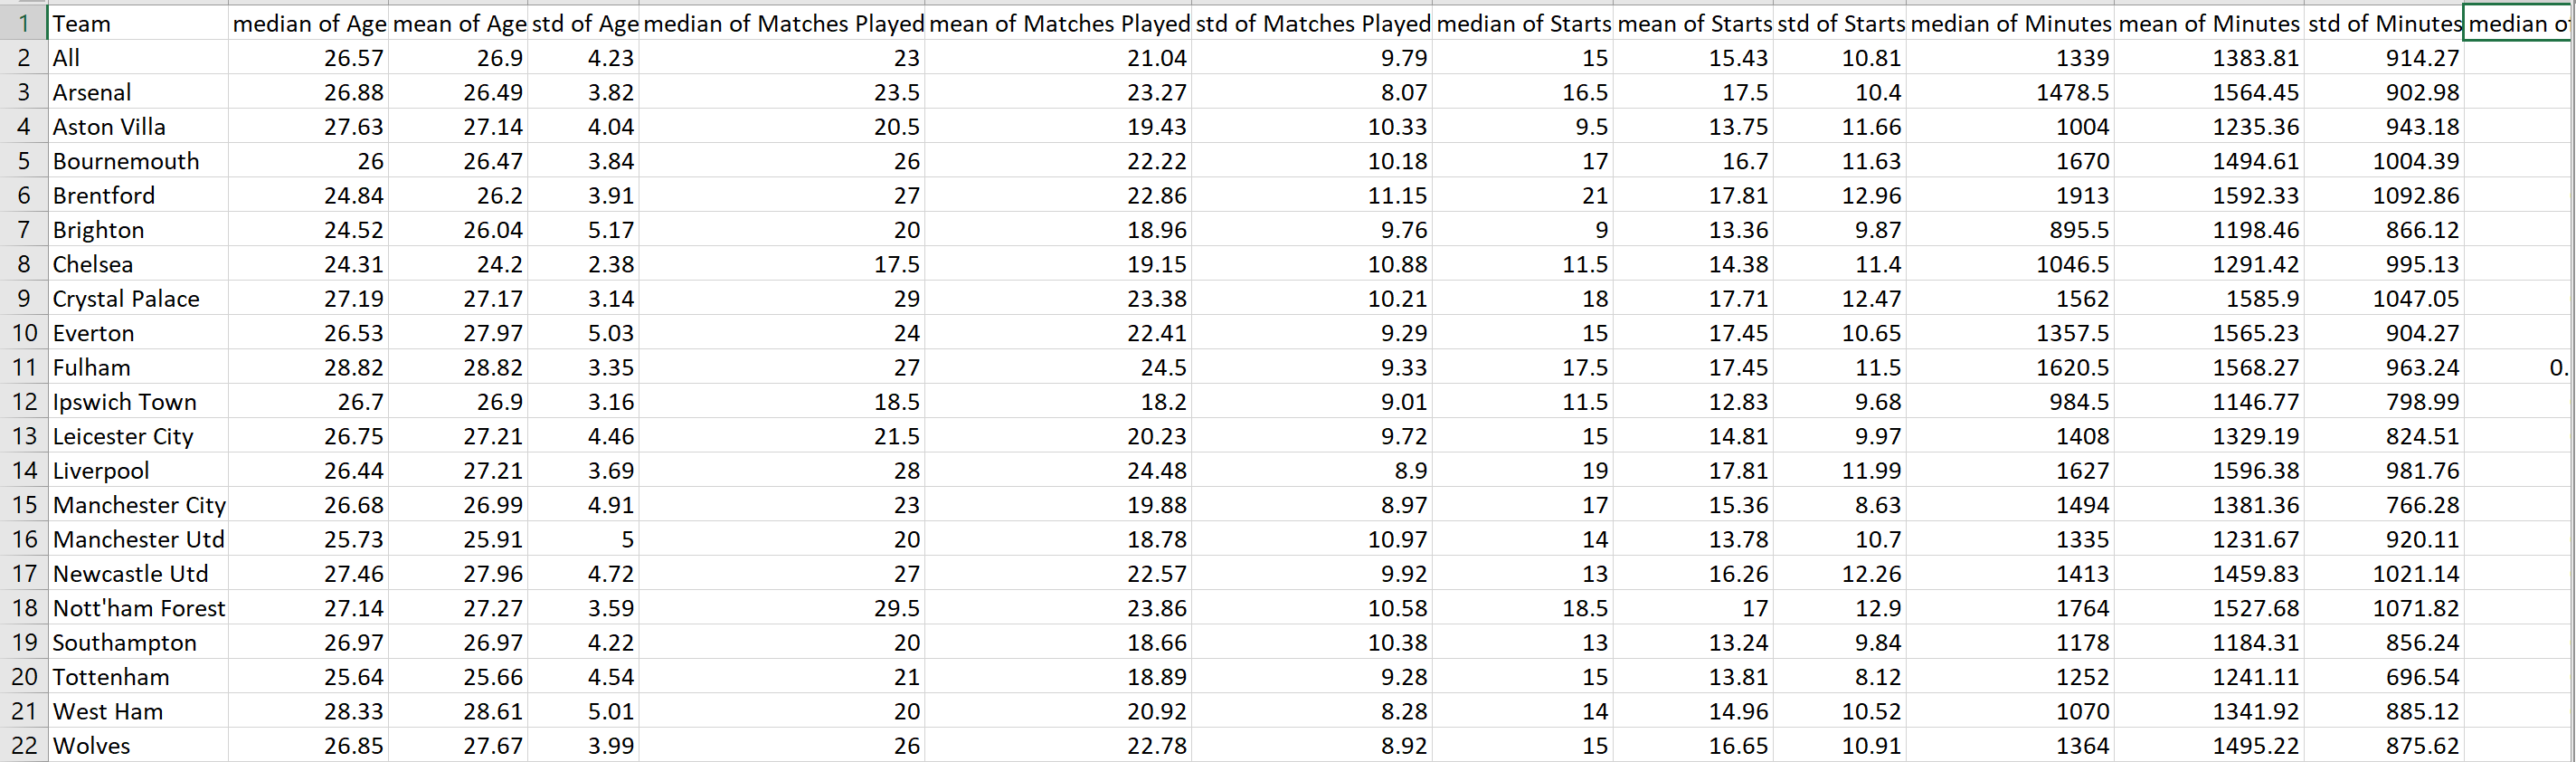
\includegraphics[width=6.5in,height=1.9166666666666667in]{media/image4.png}
    \caption{Summary statistics example}
\end{figure}

\subsection{Histogram Visualization}
Histograms were plotted for key statistics (\texttt{Goals, Assists, G/sh, Tackles, Challenges, and Blocks}) using \texttt{plot\_histogram():}
\begin{itemize}
    \item Distribution histograms for all players in the league.
    \item Separate histograms for each team.
    \item All plots were compiled into a single PDF: histograms.pdf.
\end{itemize}

\begin{figure}[H]
    \centering
    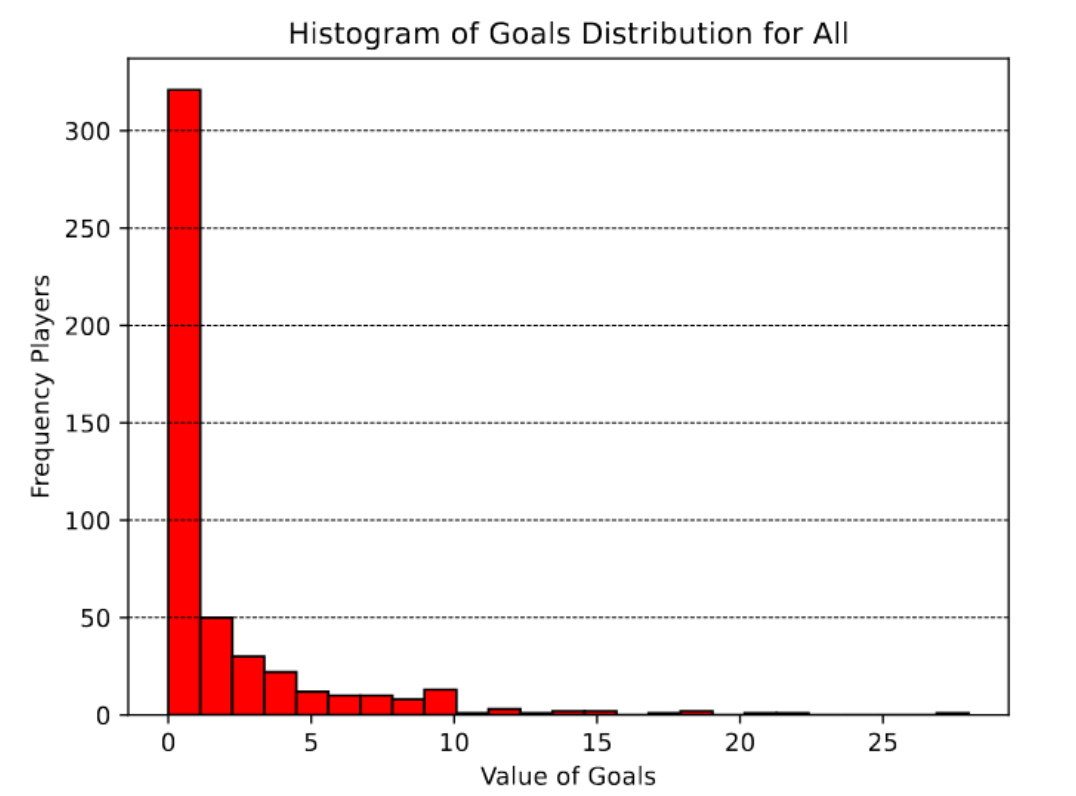
\includegraphics[width=5.557292213473316in,height=4.061097987751531in]{media/image9.png}
    \caption{Histogram example 1}
\end{figure}

\begin{figure}[H]
    \centering
    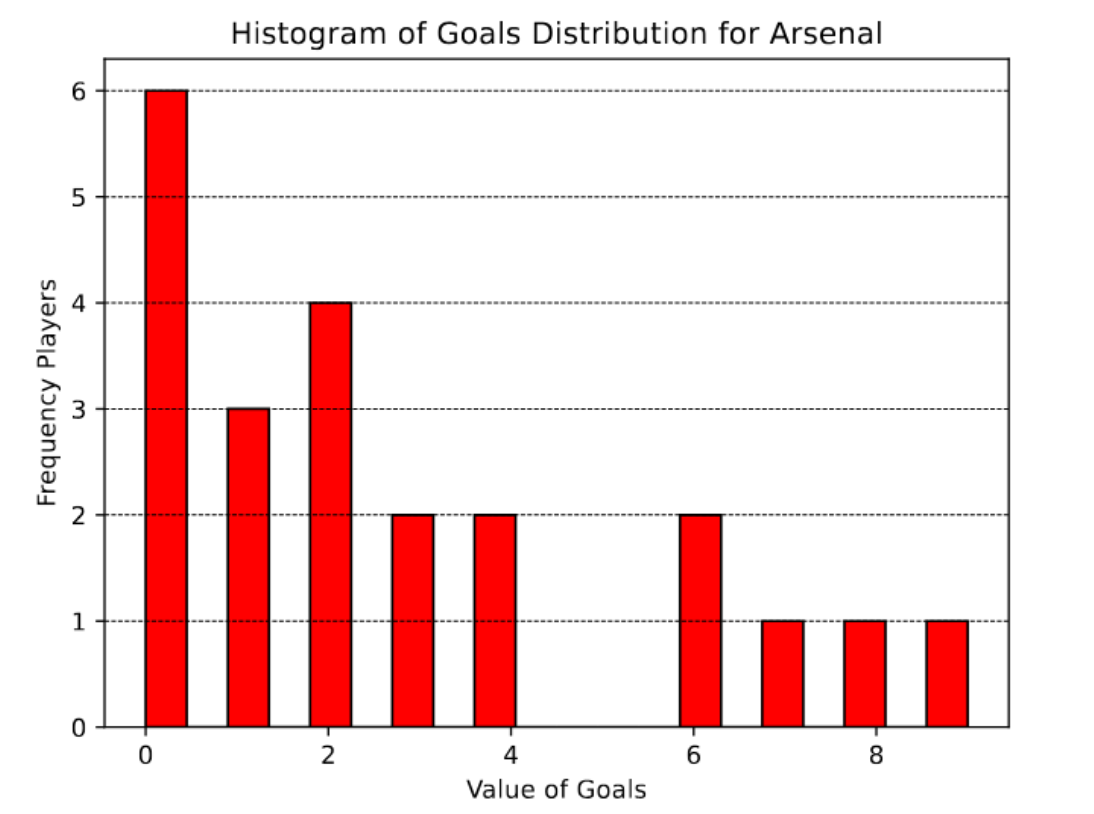
\includegraphics[width=5.755208880139983in,height=4.168293963254593in]{media/image11.png}
    \caption{Histogram example 2}
\end{figure}

\subsection{Team Performance Evaluation}
The function \texttt{identify\_team\_with\_highest\_score():}
\begin{itemize}
    \item Loads team averages from \texttt{result2.csv.}
    \item Determines which team has the highest mean for each statistic.
    \item Counts how many times each team leads across different statistics.
    \item Declares the team with the most appearances as the \textbf{best-performing team} in the league.
\end{itemize}

Example output:
\begin{itemize}
    \item Fulham has the highest Age score.
    \item Liverpool has the highest Matches Played score.
    \item Brentford has the highest Starts score.
    \item Liverpool has the highest Minutes score.
   
   => Liverpool is performing the best in the 2024-2025 Premier League season.
\end{itemize}

\section{Result}

The statistical analysis and visualizations yielded several meaningful insights regarding player and team performances during the 2024–2025 Premier League season:

\begin{itemize}
    \item \textbf{Top and Bottom 3 Players}: For each key statistic, the top 3 and bottom 3 players were identified and exported to \texttt{top\_3.txt}. This allowed for a quick overview of standout individual performances across the league.
    
    \item \textbf{Summary Statistics}: Median, mean, and standard deviation values were calculated for both the league-wide dataset and individual teams. These values were saved in \texttt{result2.csv} for further analysis or comparison.
    
    \item \textbf{Histograms}: A series of histograms were generated to visualize the distribution of important metrics such as \texttt{Goals, Assists, Shots per Goal, Tackles, Challenges,} and \texttt{Blocks.} All plots were compiled into a single PDF file: \texttt{histograms.pdf}.
    
    \item \textbf{Best Performing Team}: Based on average values across all statistics, Liverpool was identified as the best-performing team of the season. This conclusion was drawn by counting the number of statistics in which each team had the highest average.
\end{itemize}

% Phần III
\chapter{Clustering and \mbox{Dimensionality} Reduction}
\section{Objective}
This section applies machine learning techniques to group Premier League players into distinct categories based on their statistical performance using:
\begin{itemize}
    \item \textbf{K-means Clustering}.
    \item \textbf{PCA (Principal Component Analysis)} for dimensionality reduction and visualization.
\end{itemize}

\section{Tools and Libraries Used}
   \texttt{pandas:} to load, clean, and preprocess player data, including scaling and handling missing values.
   
   \texttt{matplotlib:} to visualize data distributions, Elbow and Silhouette methods, and PCA-clustered player groups.
   
   \texttt{sklearn:}  used for clustering and evaluation tasks including: KMeans, StandardScaler, silhouette\_score, PCA

\section{Methodology}
\subsection{Data Preprocessing}
\begin{itemize}
    \item The dataset from \texttt{result.csv} was loaded.
    \item Age was transformed from \texttt{"years-days"} format to float (\texttt{23-45 → 23.12}).
    \item All non-numeric and missing values \texttt{"N/a"} were converted to 0 to enable numerical processing.
    \item \texttt{StandardScaler} was used to normalize all numerical features before clustering.
\end{itemize}

\subsection{Optimal K Determination}
To choose the appropriate number of clusters (k) for K-means, two methods were employed:

\subsubsection{Elbow Method}
\begin{itemize}
    \item Plotted number of clusters (k) vs. inertia (within-cluster sum of squares).
    \item A clear "elbow" in the curve indicates the optimal k.
\end{itemize}

\subsubsection{Silhouette Method}
\begin{itemize}
    \item Calculated silhouette scores for each k to measure cohesion/separation.
    \item The higher the score, the better the clustering quality.
\end{itemize}

\subsubsection{Result}
\begin{figure}[H]
    \centering
    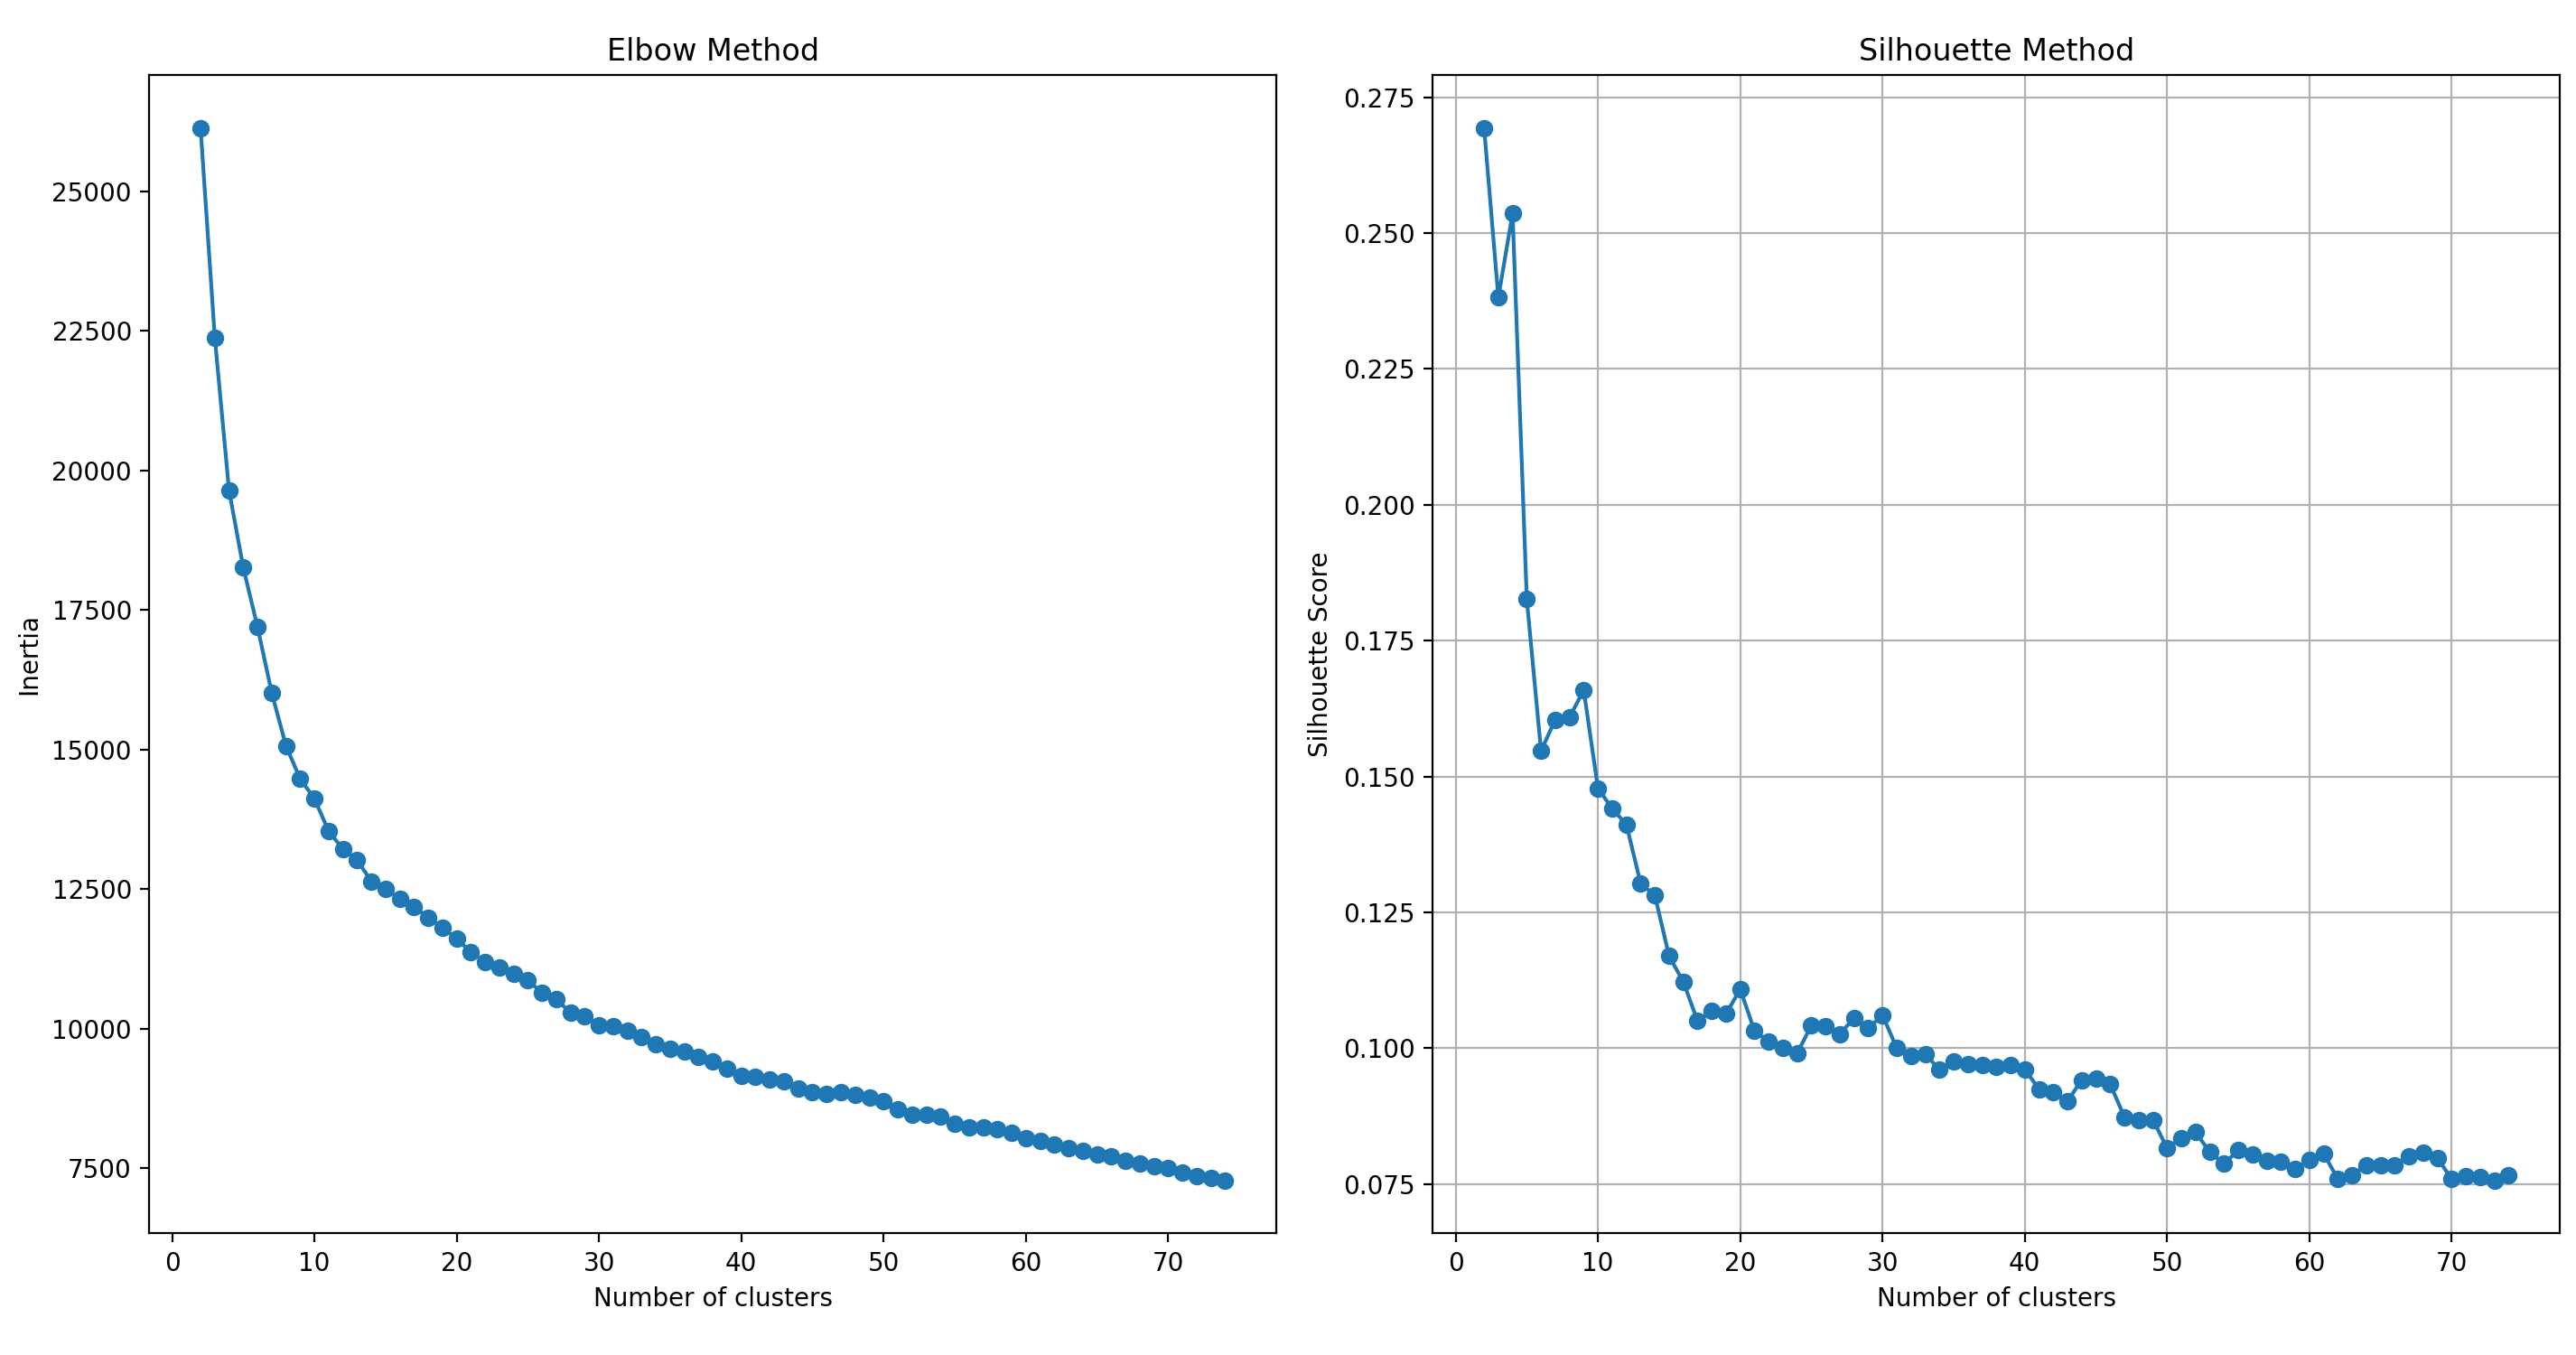
\includegraphics[width=6.5in,height=3.4166666666666665in]{media/image3.png}
\end{figure}

\begin{figure}[H]
    \centering
    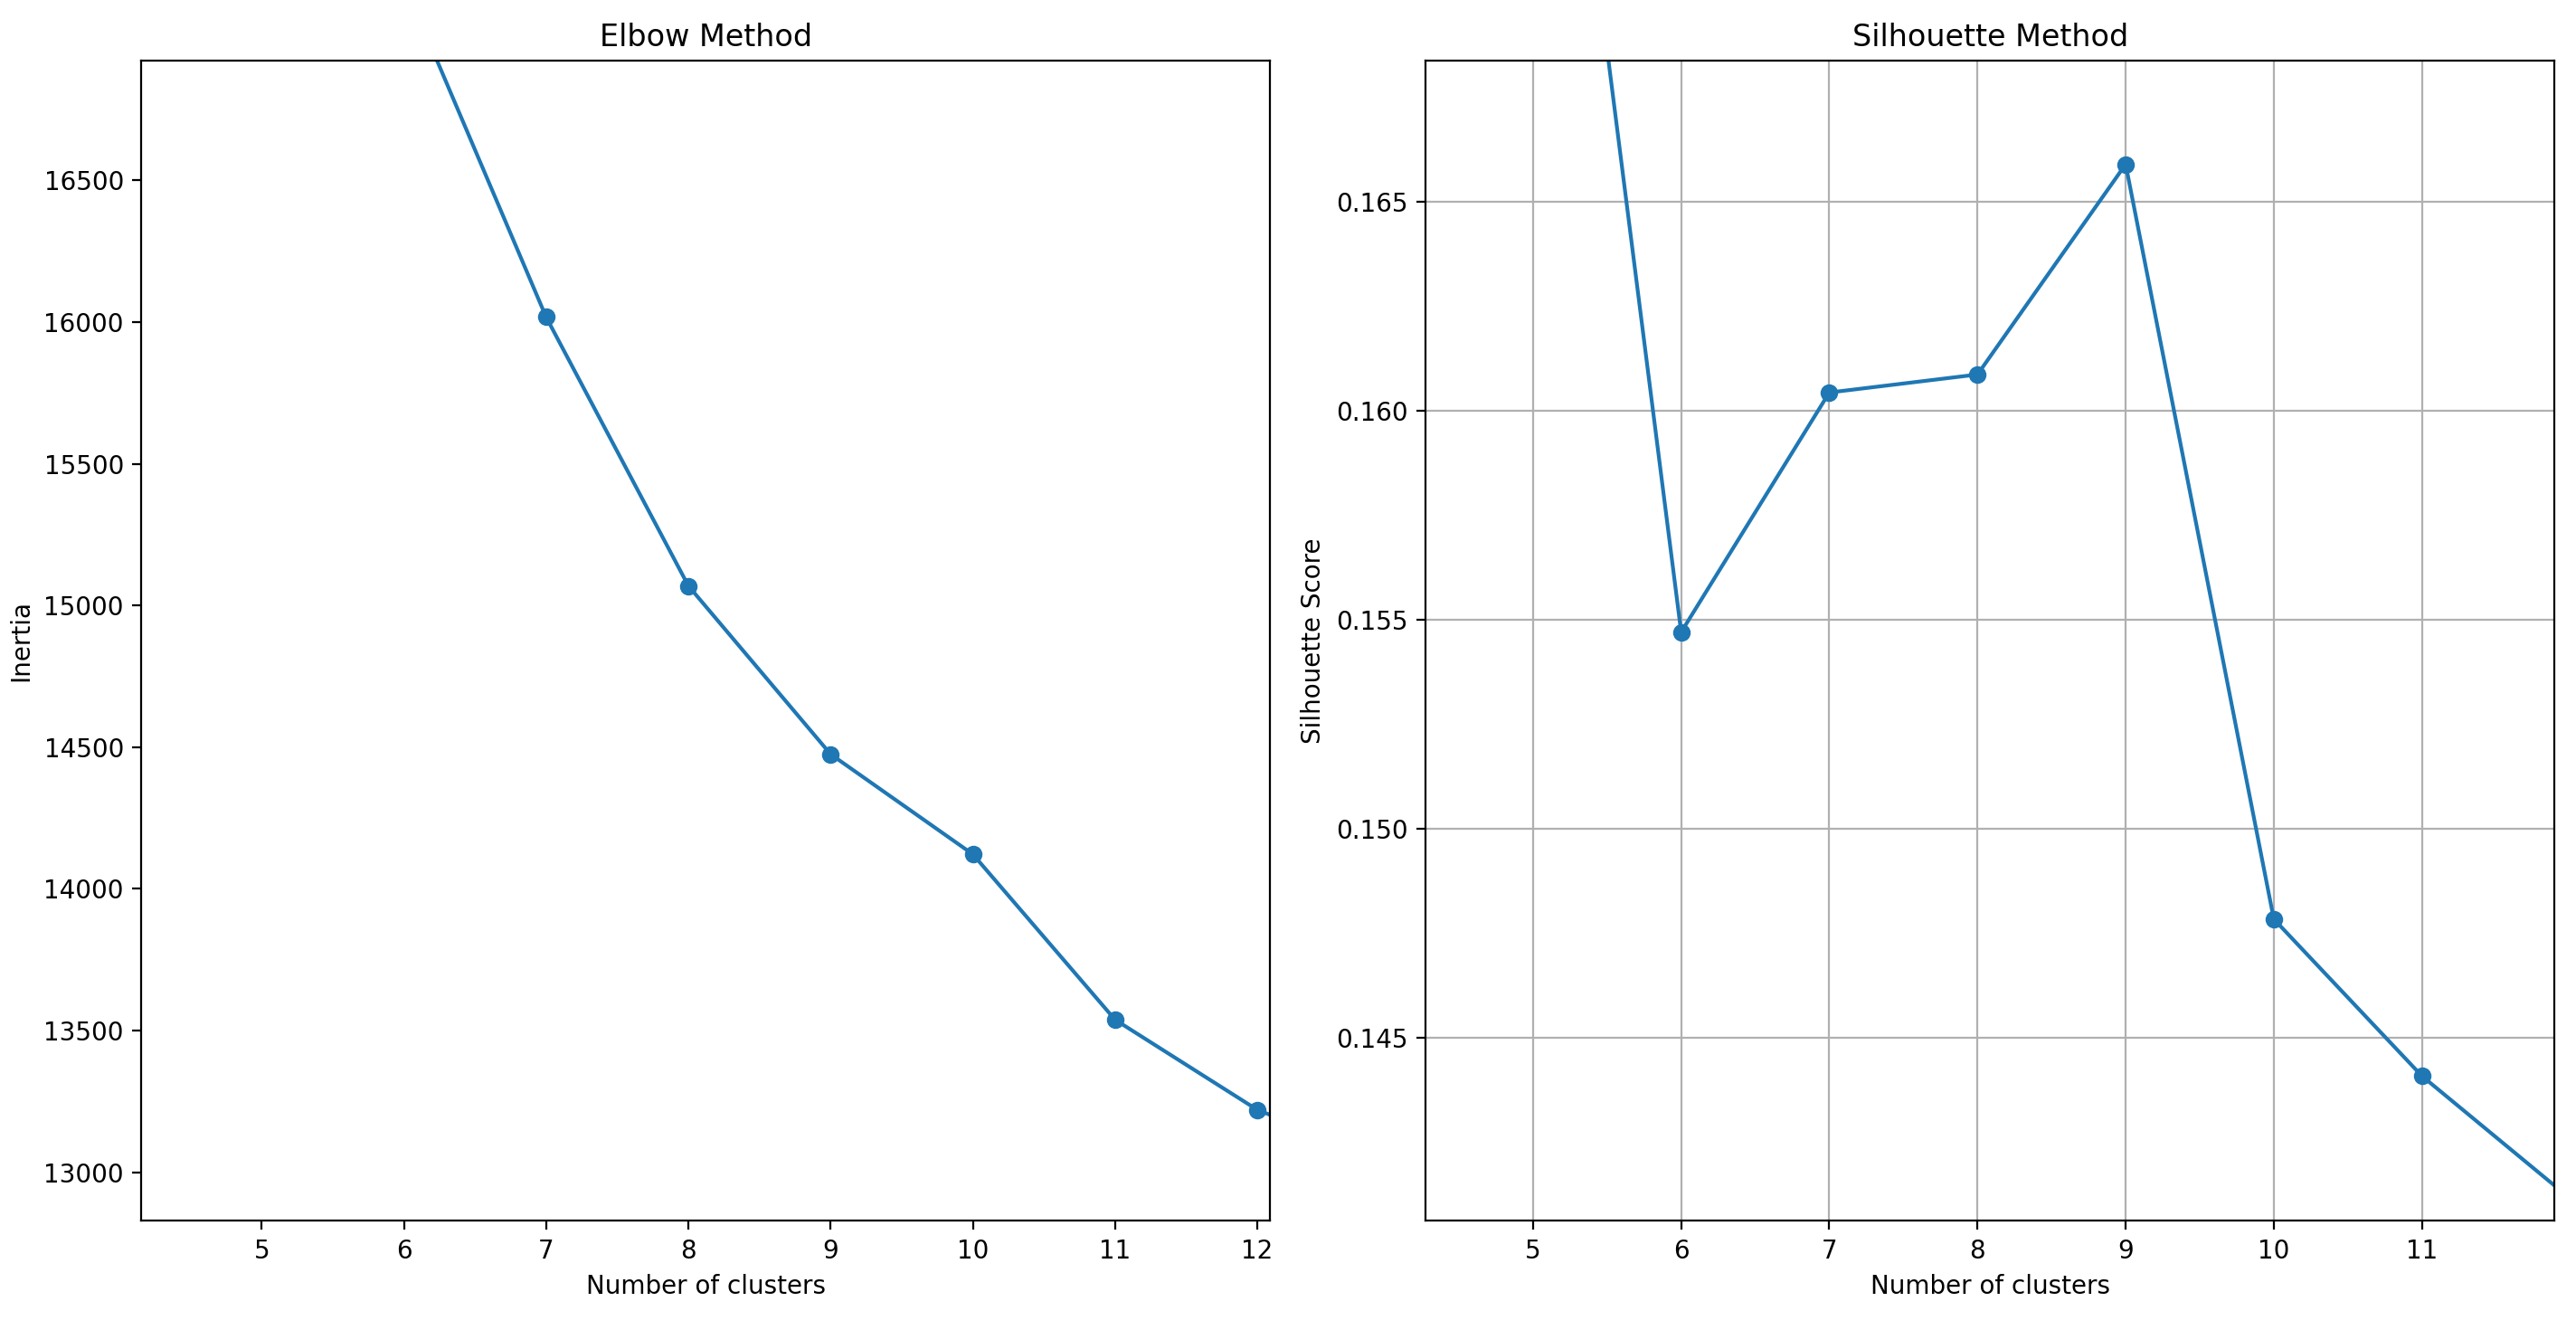
\includegraphics[width=6.5in,height=3.4444444444444446in]{media/image12.png}
    \caption{Elbow method and Silhouette method result}
\end{figure}

Based on both plots, the best value of k was estimated in the range \textbf{6 to 10}.

\subsection{K-Means Clustering and Dimensionality Reduction with PCA}
The function \texttt{run\_kmeans\_and\_plot():}
\begin{itemize}
    \item For k = 6, 7, 8, 9, KMeans clustering was performed:
    \begin{itemize}
        \item The KMeans algorithm from sklearn.cluster is fitted to the scaled player statistics.
        \item Principal Component Analysis (PCA) is used to reduce the dataset to 2 principal components (PC1 and PC2).
        \item A scatter plot is created for each k value, showing how players are grouped in 2D space based on PCA.
    \end{itemize}
\end{itemize}

\begin{figure}[H]
    \centering
    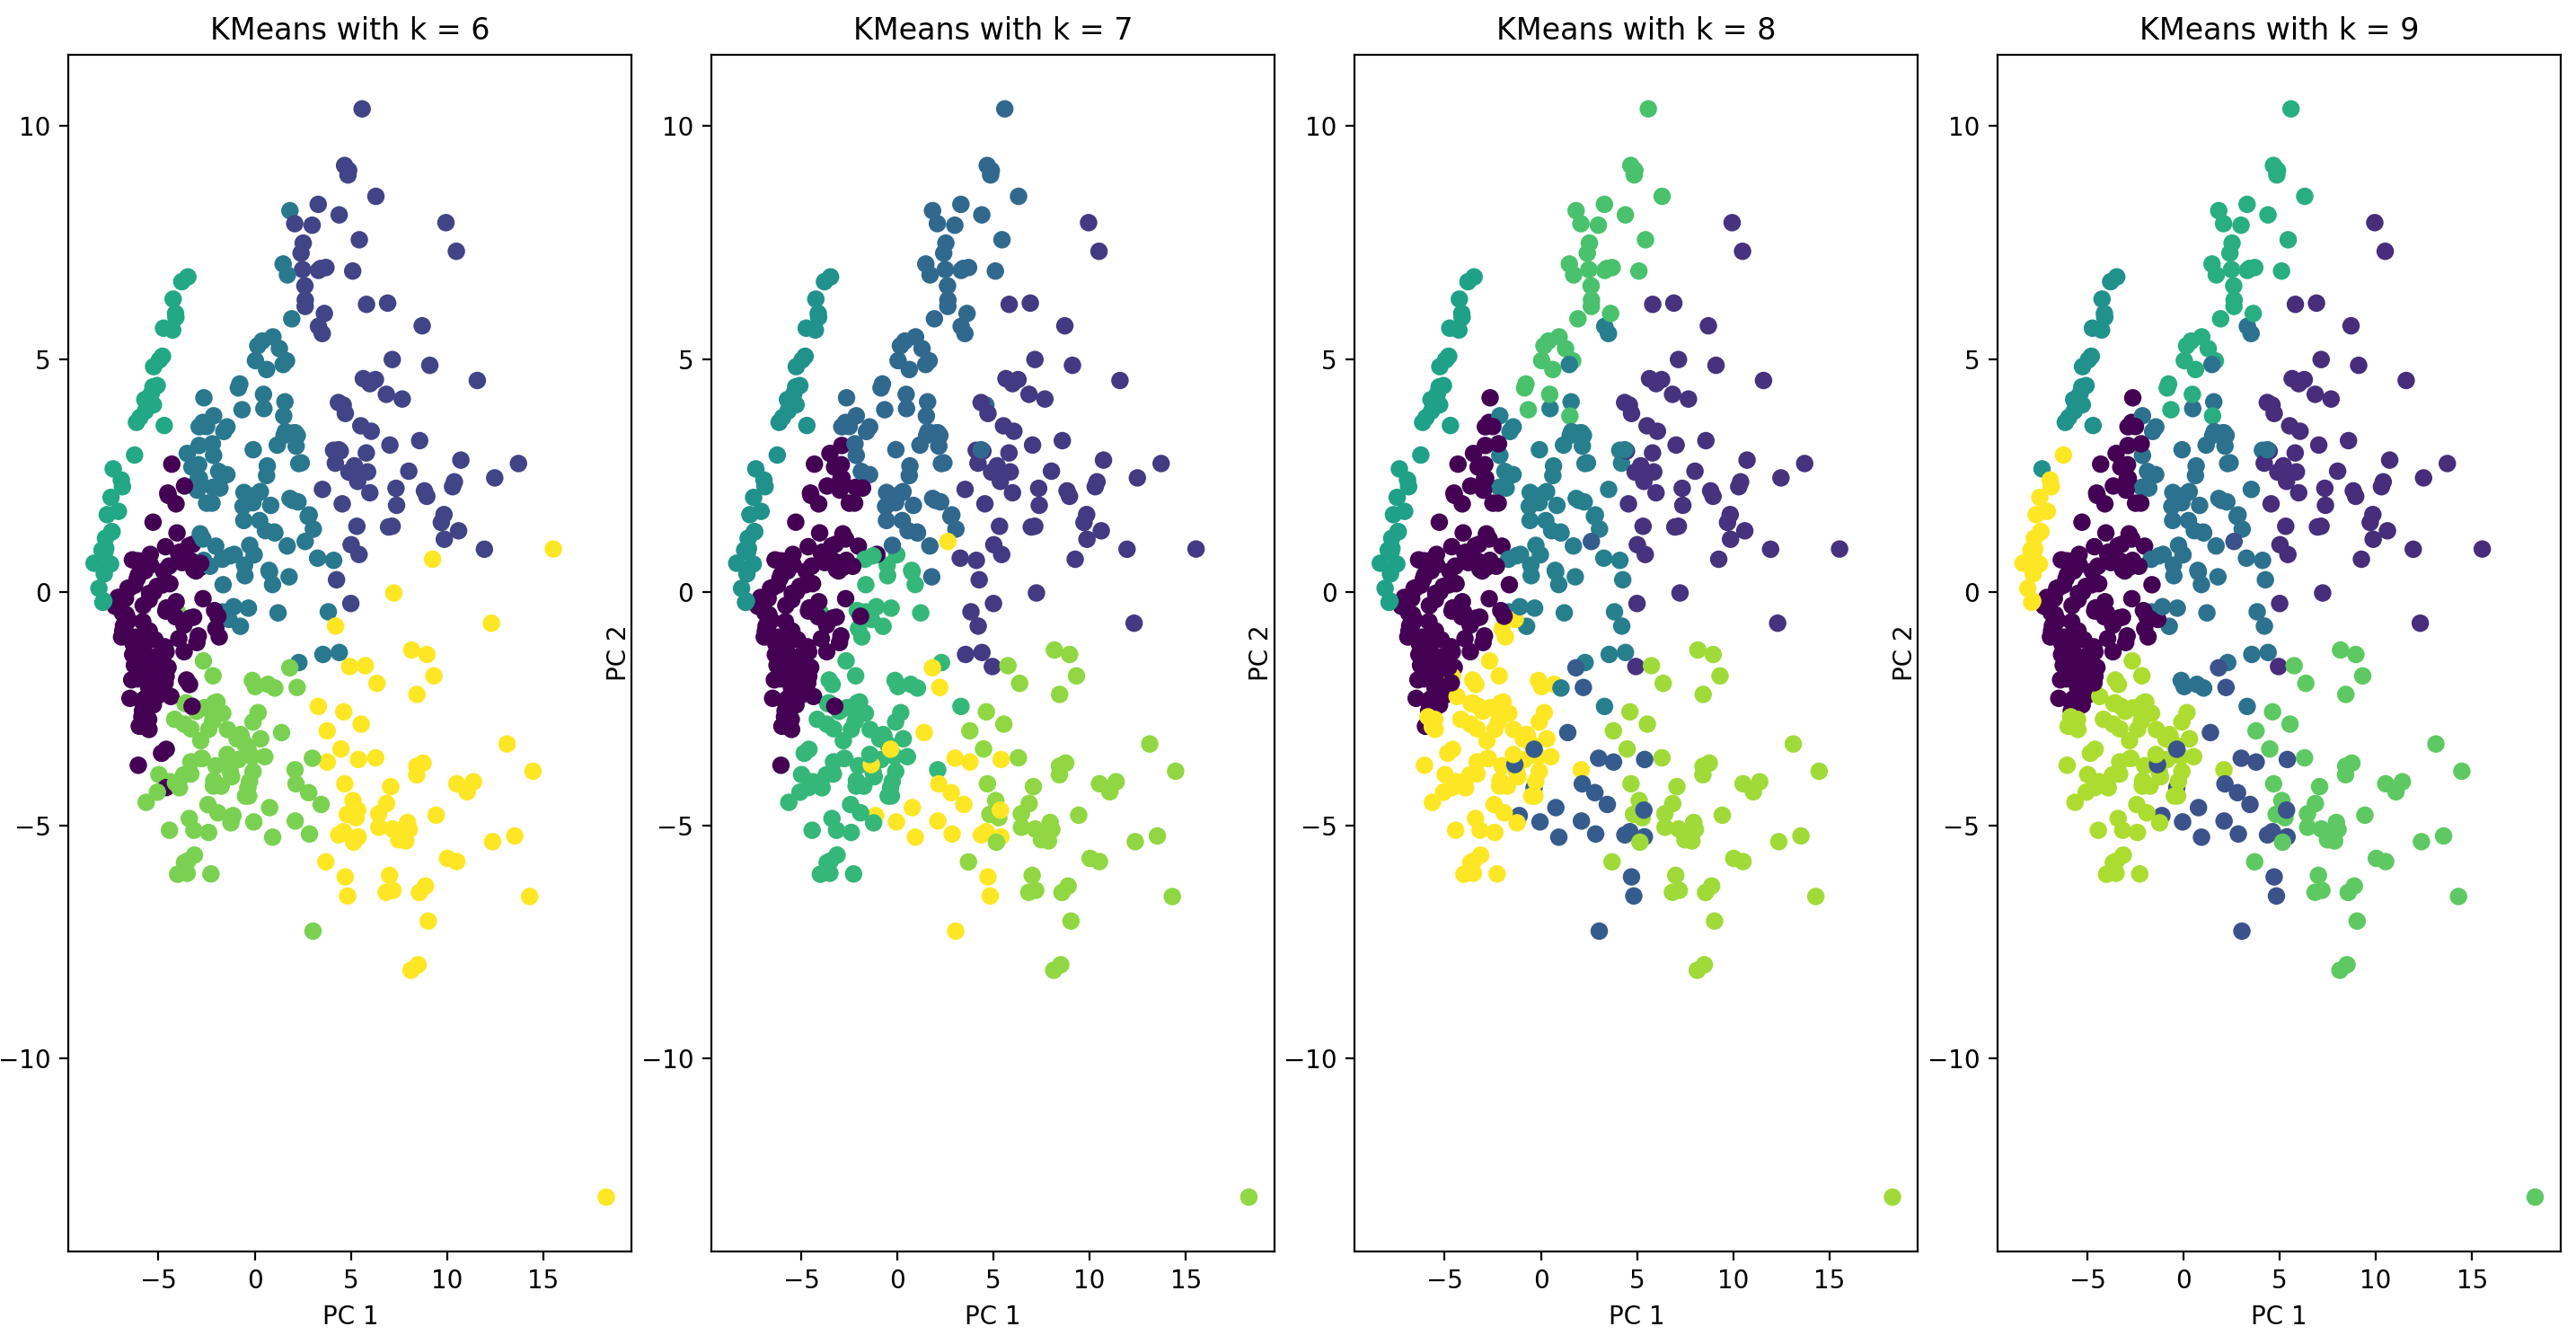
\includegraphics[width=6.5in,height=3.625in]{media/image13.png}
    \caption{K-means clustering results}
\end{figure}

\section{Result}
The visualizations showed that \textbf{k = 8} provides relatively distinct and well-separated clusters. All elements clearly and consistently belong to their respective clusters.

\begin{figure}[H]
    \centering
    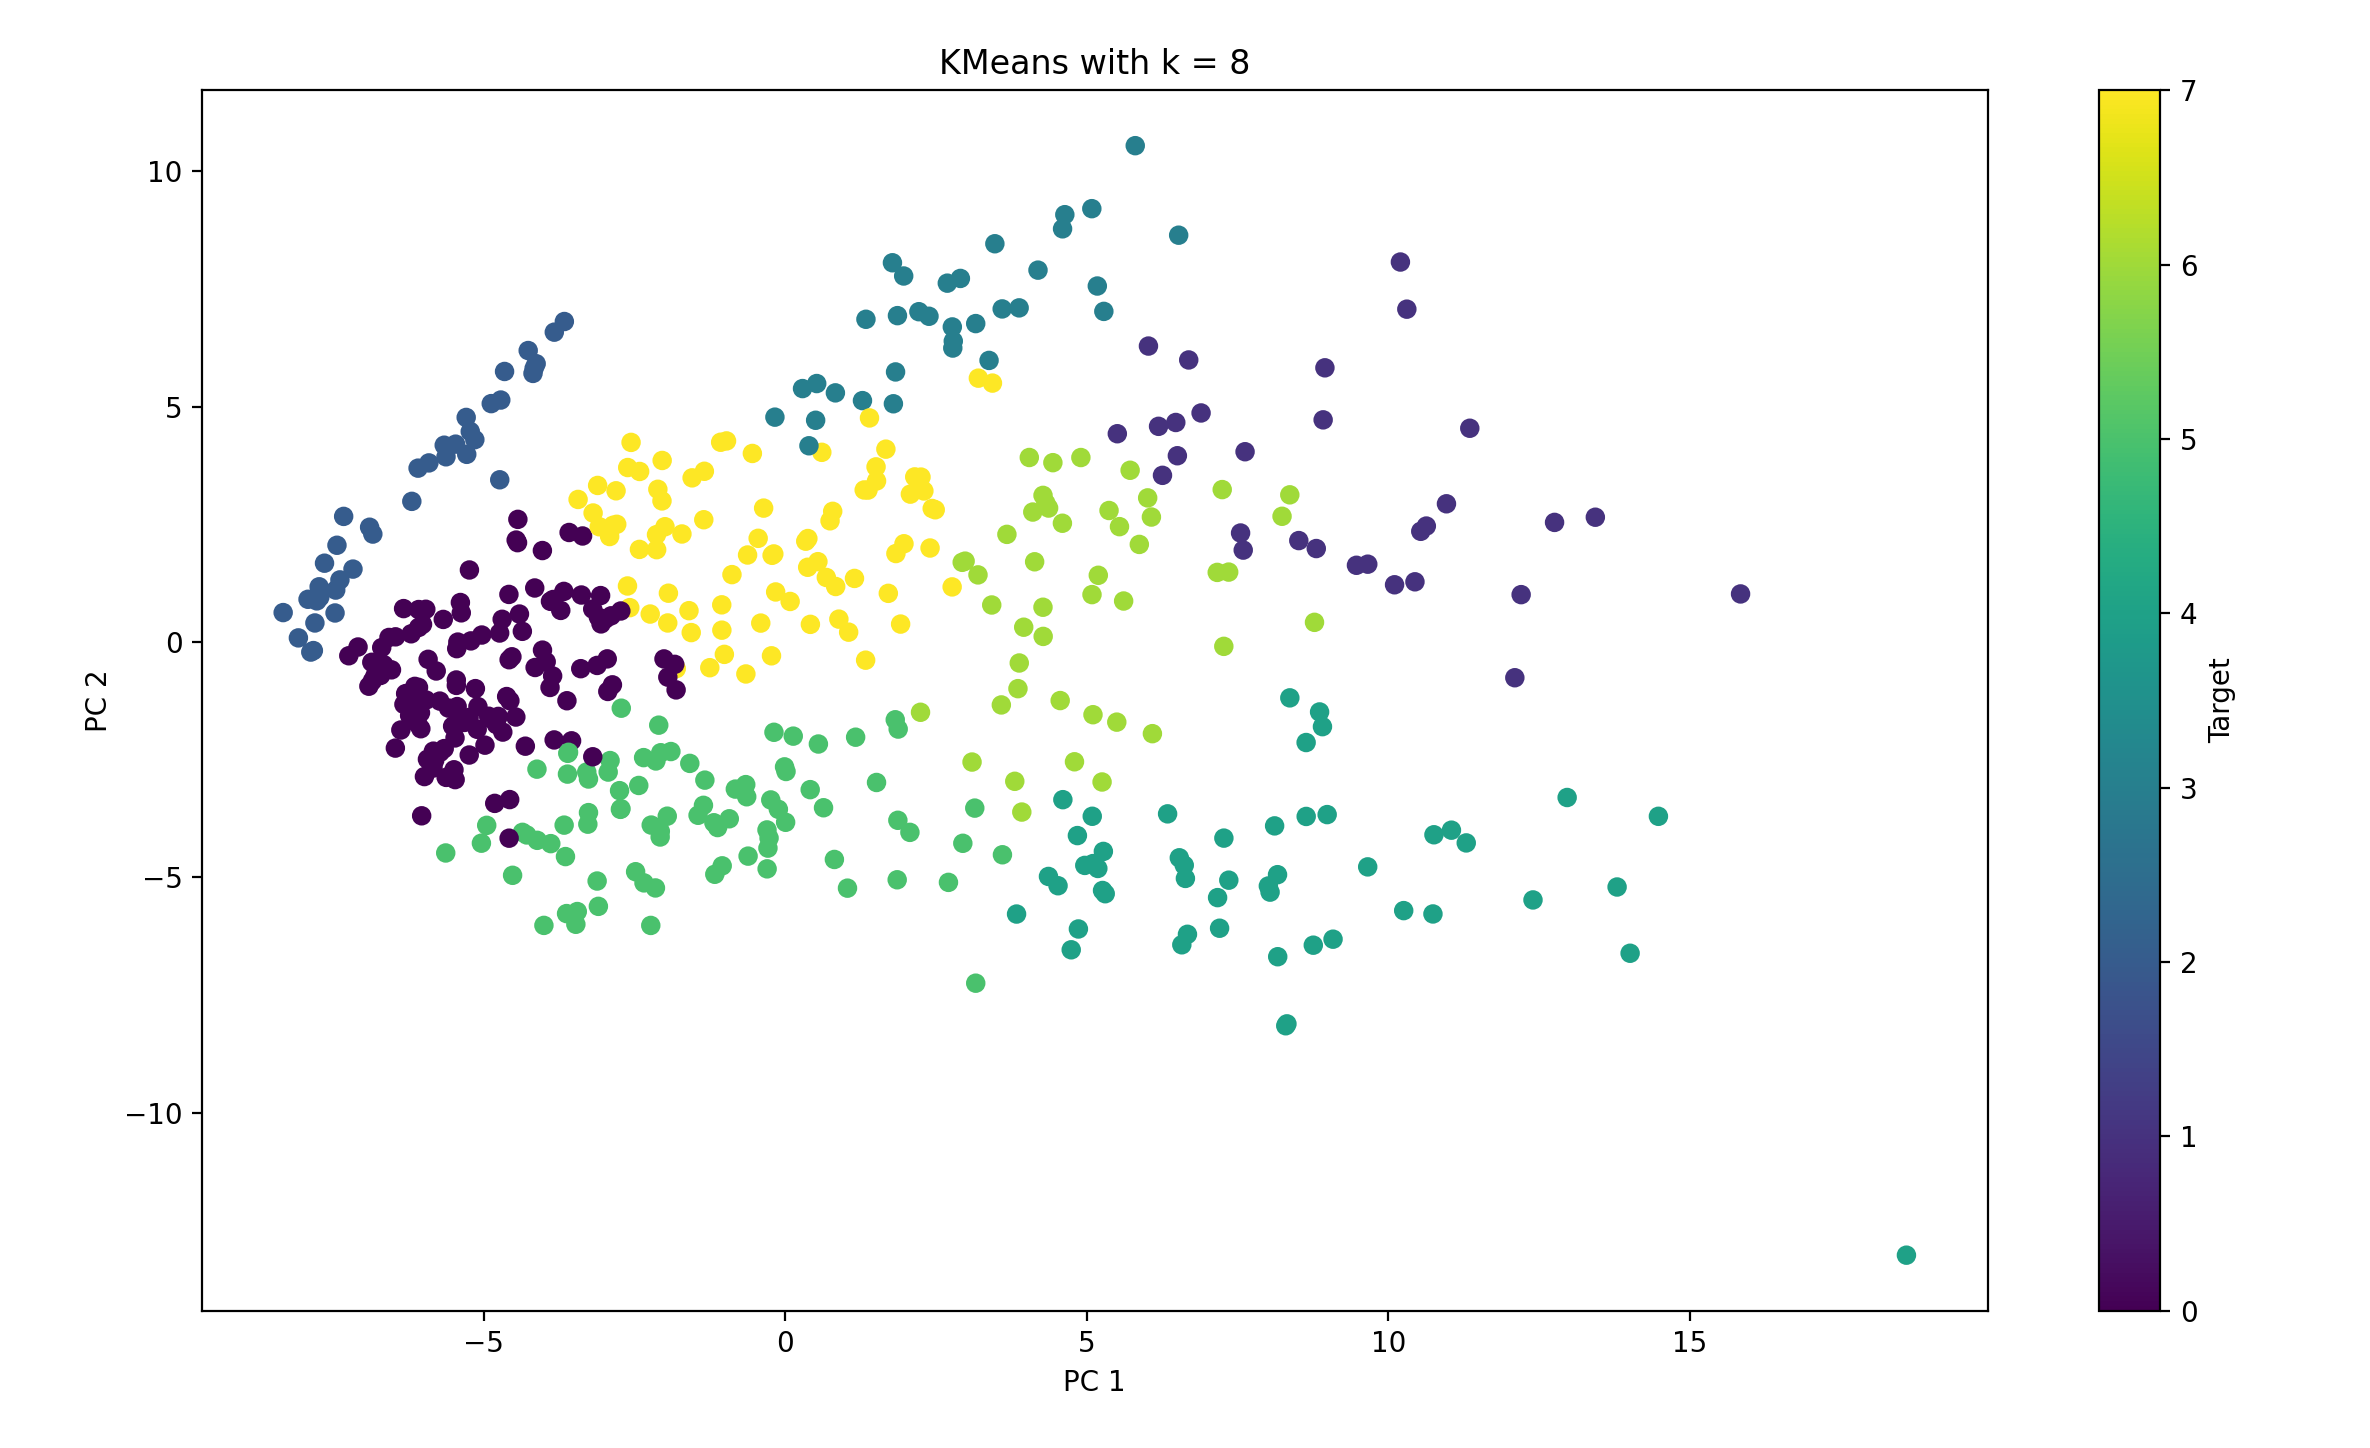
\includegraphics[width=6.088542213473316in,height=3.661352799650044in]{media/image8.png}
    \caption{Final clustering result with k=8}
\end{figure}

% Phần IV
\chapter{Player Transfer Values and Value Estimation}
\section{Objective}
The objective of this section was to:
\begin{itemize}
    \item Collect estimated transfer values for Premier League players from \href{https://footballtransfers.com}{FootballTransfers.com}.
    \item Match these values with previously collected player statistics (from \href{https://fbref.com/en/}{FBref.com}).
    \item Propose a method to estimate player value based on performance metrics.
\end{itemize}

\section{Tools and Libraries Used}
   \texttt{requests:} to send HTTP POST requests to football-related APIs for retrieving transfer and player search data.
   
   \texttt{pandas:} to reading, manipulating, filtering, and merging tabular data.
   
   \texttt{rapidfuzz:} utilized for fuzzy string matching to align player names from different data sources.
   
   \texttt{unidecode:} to normalize player names by removing accents and special characters.
   
   \texttt{sklearn:} for machine learning algorithms and model evaluation.
   
   \texttt{numpy:} for numerical computations and array operations.
   
   \texttt{seaborn:} for creating attractive and informative statistical graphics.
   
   \texttt{matplotlib:} for plotting graphs and visualizing data.

\section{Methodology}
\subsection{Data Collection}
\subsubsection{Two APIs were used:}
\begin{itemize}
    \item Player values API: queried across 22 pages to retrieve the top ~500 most valuable players in the EPL.
    \item Search API: used for special cases where players were not listed in the top ranks.
\end{itemize}

\subsubsection{Data Collection from API}
\begin{itemize}
    \item Sent paginated POST requests (pages 1 to 22) to retrieve top ~500 most valuable players.
    \item Extracted \texttt{player\_name, age, team\_short\_name}, and \texttt{estimated\_value.}
\end{itemize}

\subsubsection{Filtering FBref Data}
\begin{itemize}
    \item Loaded \texttt{result.csv}, which contains FBref data.
    \item Filtered players with more than 900 minutes played.
\end{itemize}

\subsubsection{Name Normalization and Matching}
\begin{itemize}
    \item Created a simplified \texttt{name\_key} by removing accents and sorting name tokens to reduce matching ambiguity.
    \item Used \texttt{RapidFuzz} to match \texttt{player\_name} from FootballTransfers with Player from FBref using fuzzy ratio scores.
\end{itemize}

\subsubsection{Handling Missing Matches}
\begin{itemize}
    \item Identified unmatched players after fuzzy matching.
    \item Queried the \textbf{Search API} for these exception cases to manually retrieve their transfer values.
    \item Merged results with matched players.
\end{itemize}

\subsubsection{Result}
The final merged dataset includes:
\begin{itemize}
    \item Player, Team, and Transfer Value
    \item Saved as \texttt{player\_transfer\_values.csv}
\end{itemize}

\begin{figure}[H]
    \centering
    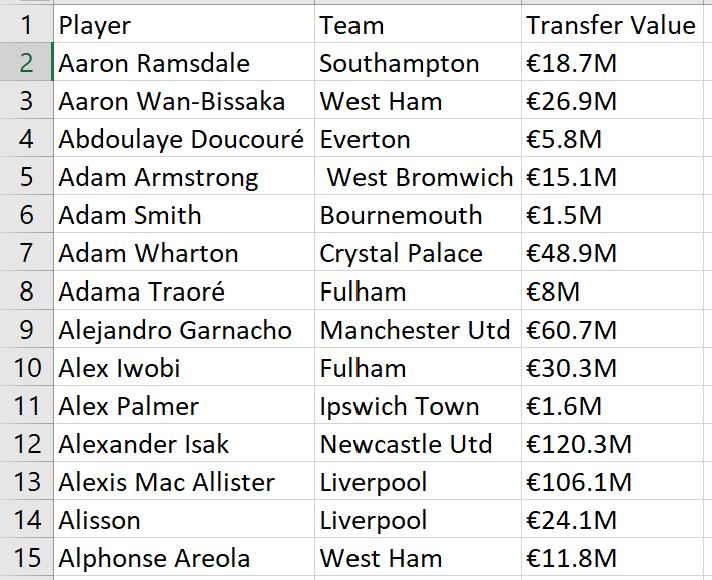
\includegraphics[width=5in,height=3in]{media/image2.png}
    \caption{Example of transfer value}
\end{figure}

\subsection{Feature Selection and Modeling}
\subsubsection{Data collection}
\begin{itemize}
    \item \textbf{Player Performance Data} was loaded from \texttt{result.csv}, containing detailed statistics scraped from \href{https://fbref.com/en/}{FBref.com}. Only players with more than \textbf{900 minutes played} were retained to ensure data reliability.
    \item \textbf{Transfer Value Data} was loaded from \texttt{player\_transfer\_values.csv}, created using a custom script that scrapes estimated market values from \href{https://footballtransfers.com}{FootballTransfers.com}.
    \item The two datasets were \textbf{merged} on the \texttt{Player name} field to associate performance data with corresponding transfer values.
    \item Placeholder values such as \texttt{'N/a'} were replaced with \texttt{NaT} to ensure consistent data types and facilitate downstream processing.
\end{itemize}

\subsubsection{Statistics}
\begin{itemize}
    \item The merged dataset consists of \textbf{303 rows and 79 columns} (df.shape), covering a wide range of player performance metrics.
    \item A review of missing data indicates that several features contain a significant proportion of null values.
    \item The dataset also contains \textbf{17 categorical features}, including Player, Team, Position, etc.
\end{itemize}

\subsubsection{Data preprocessing}
To prepare the dataset for modeling, the following preprocessing steps were applied:
\begin{itemize}
    \item \textbf{Outlier Removal}: The player Mohamed Salah was removed from the dataset.
    \begin{figure}[H]
        \centering
        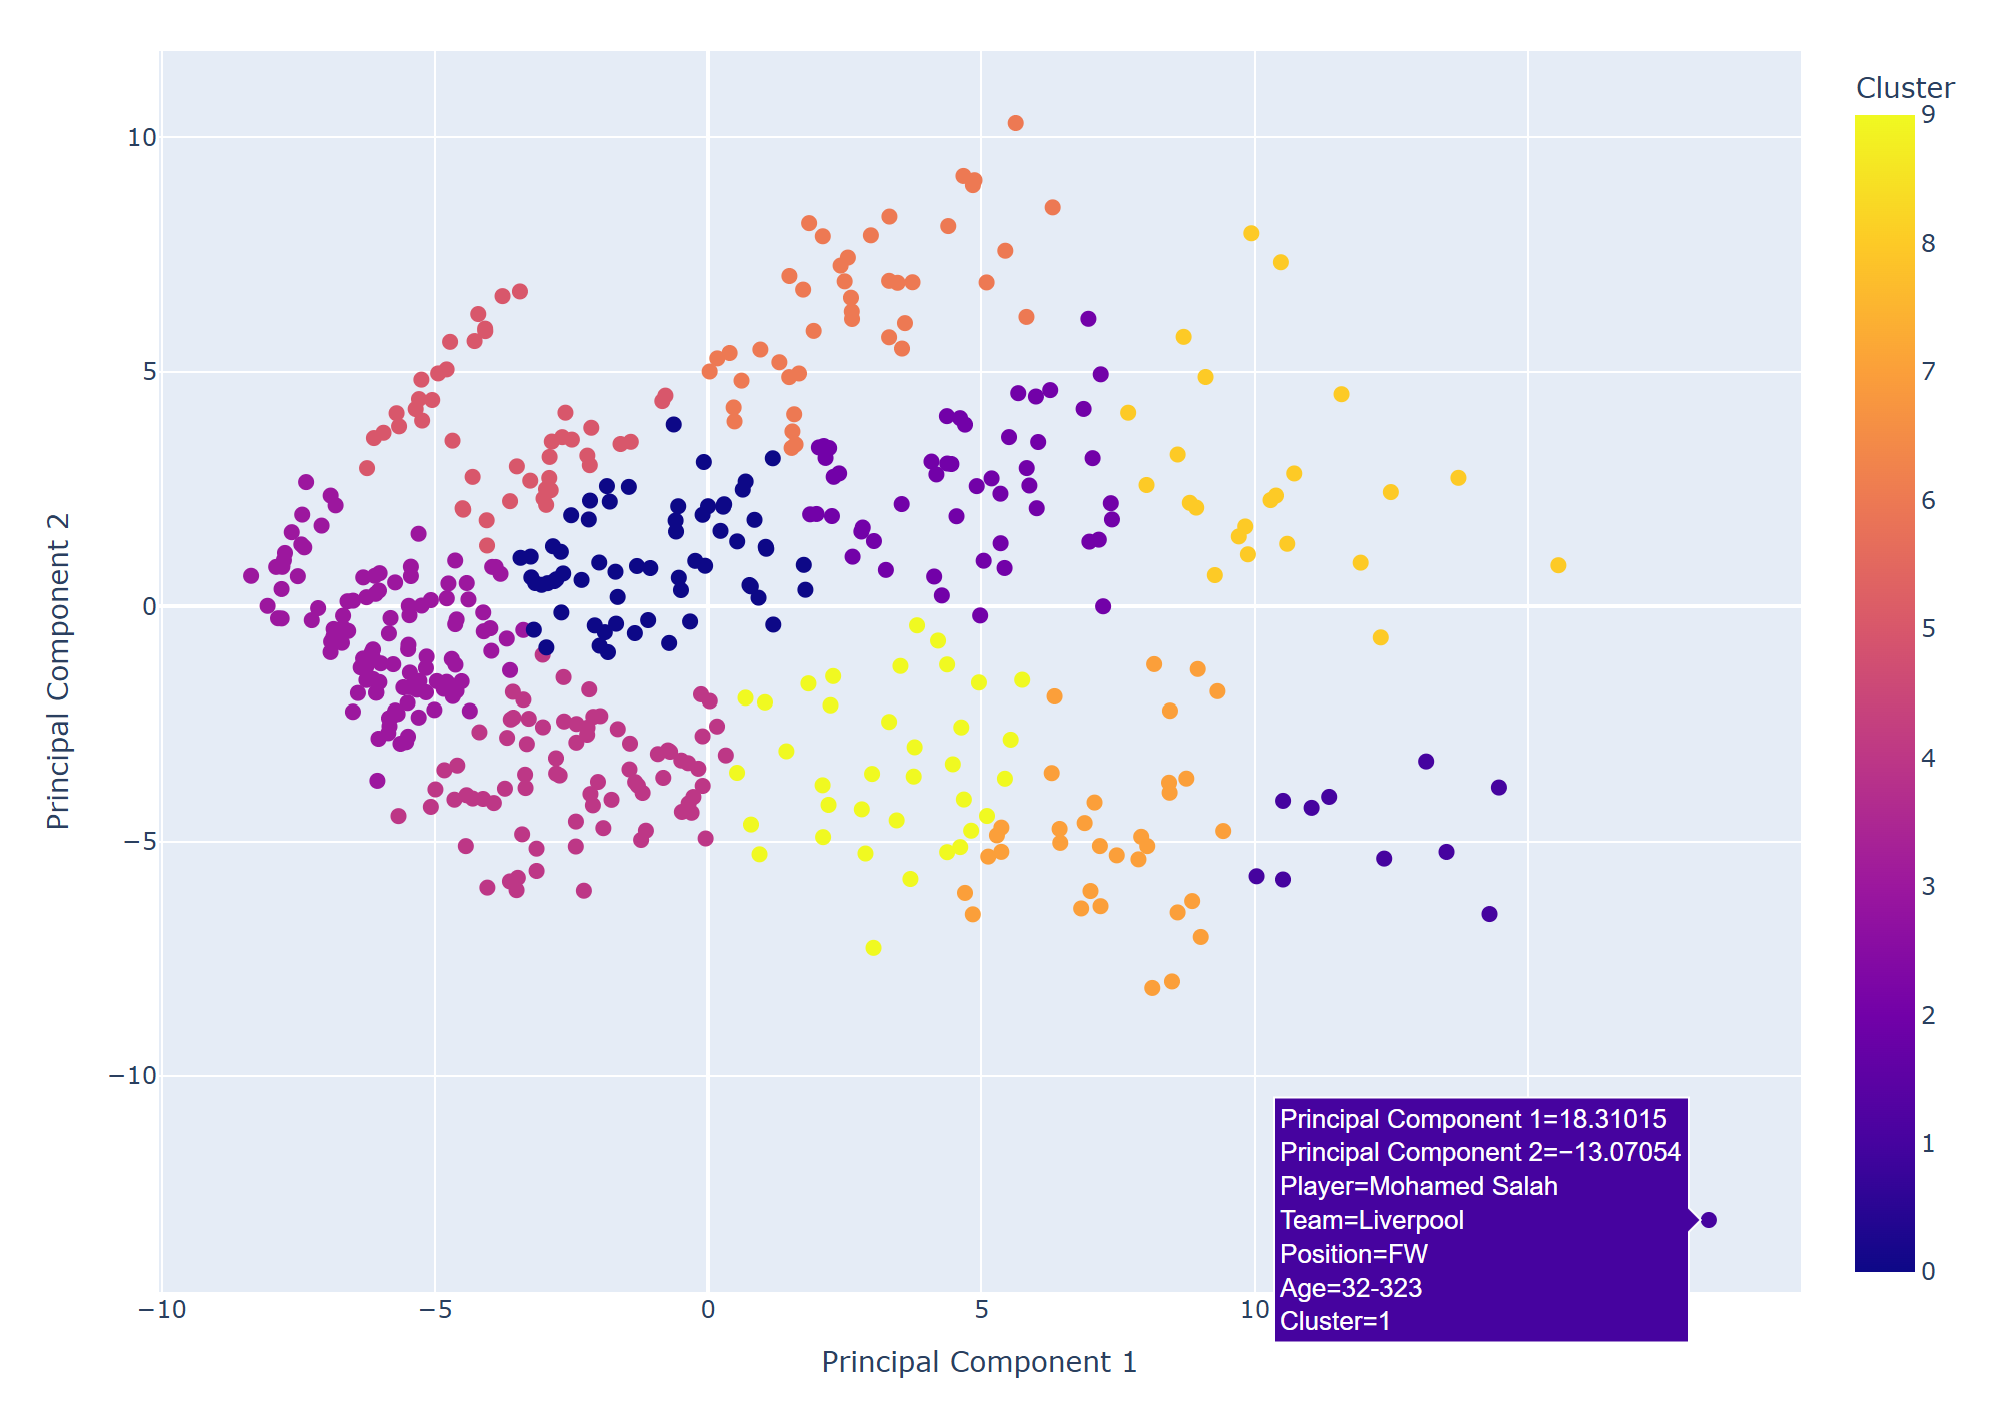
\includegraphics[width=5in,height=3in]{media/image16.png}
        \caption{PCA plot}
    \end{figure}
    \item \textbf{Handling Missing Data}:
    \begin{itemize}
        \item Features with excessive missing values were dropped.
        \item For partially missing features, missing values were imputed using the column mean.
    \end{itemize}
    \item \textbf{Feature Transformation}:
    \begin{itemize}
        \item Age was converted from a string format to a decimal representation.
        \item Transfer Value was cleaned and converted to float.
    \end{itemize}
    \item \textbf{Data Type Conversion}: Numerical conversion was applied to various features.
    \item \textbf{Categorical Encoding}: Categorical features were encoded using Label Encoding.
    \item \textbf{Feature Reduction}: The Position column was removed.
\end{itemize}

\subsubsection{Data visualization}
\begin{itemize}
    \item \textbf{Correlation Matrix Calculation}: Computed using the .corr() method.
    \item \textbf{Heatmap Visualization}: Using coolwarm color map to represent correlation strength.
\end{itemize}

\begin{figure}[H]
    \centering
    \includegraphics[width=6.5in,height=4.388888888888889in]{media/image6.png}
    \caption{Correlation heatmap}
\end{figure}

\subsubsection{Model building}
\paragraph{Choose important features for train model (Features Selection)}
\begin{itemize}
    \item Step 1: Correlation with \texttt{Transfer Value} - Features with absolute correlation > 0.2 were retained.
    \item Step 2: Multicollinearity Reduction - Features with pairwise correlation > 0.9 were dropped.
    \item Step 3: Final Feature Set - Important features were identified based on correlation.
\end{itemize}

\paragraph{Split data train and test}
\begin{itemize}
    \item 80\% of the data used to train the model.
    \item 20\% of the data held out for testing.
    \item Training set size: 241
    \item Test set size: 61
\end{itemize}

\paragraph{Create model and train}~\\
\noindent - The following regression models were considered:
\begin{itemize}
    \item Linear Regression
    \item Random Forest Regressor
    \item Gradient Boosting Regressor
    \item K-Nearest Neighbors Regressor
    \item AdaBoost Regressor
    \item Decision Tree Regressor
\end{itemize}

- Evaluation Metrics:
\begin{itemize}
    \item R² Score (Train \& Test)
    \item Mean Squared Error (MSE)
    \item Root Mean Squared Error (RMSE)
    \item Mean Absolute Error (MAE)
    \item Training Time
    \item Prediction Time
\end{itemize}

\begin{figure}[H]
    \centering
    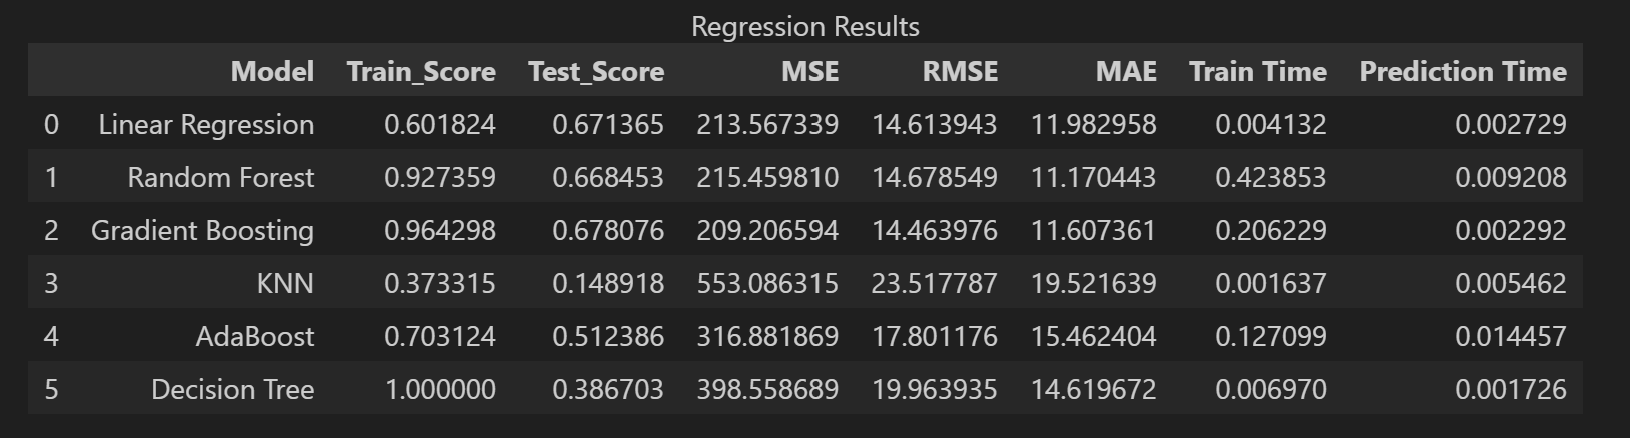
\includegraphics[width=0.8\textwidth]{media/image15.png}
    \caption{Comparison of regression models based on evaluation metrics}
    \label{fig:regression-comparison}
\end{figure}

Based on the evaluation, \textbf{Linear Regression} was chosen as the best model for the regression task.

\subsubsection{Model evaluation}
\paragraph{Evaluation Metrics}
\begin{itemize}
    \item Train R²: 0.60
    \item Test R²: 0.67
    \item MAE: 11.98
\end{itemize}

\paragraph{Cross-Validation}
5-fold cross-validation was applied using the R² metric:
\begin{itemize}
    \item Cross-validated R² scores: [0.6290007  0.44727447 0.544364   0.45966905 0.41957632]
    \item Mean CV R²: 0.50
\end{itemize}

\begin{figure}[H]
    \centering
    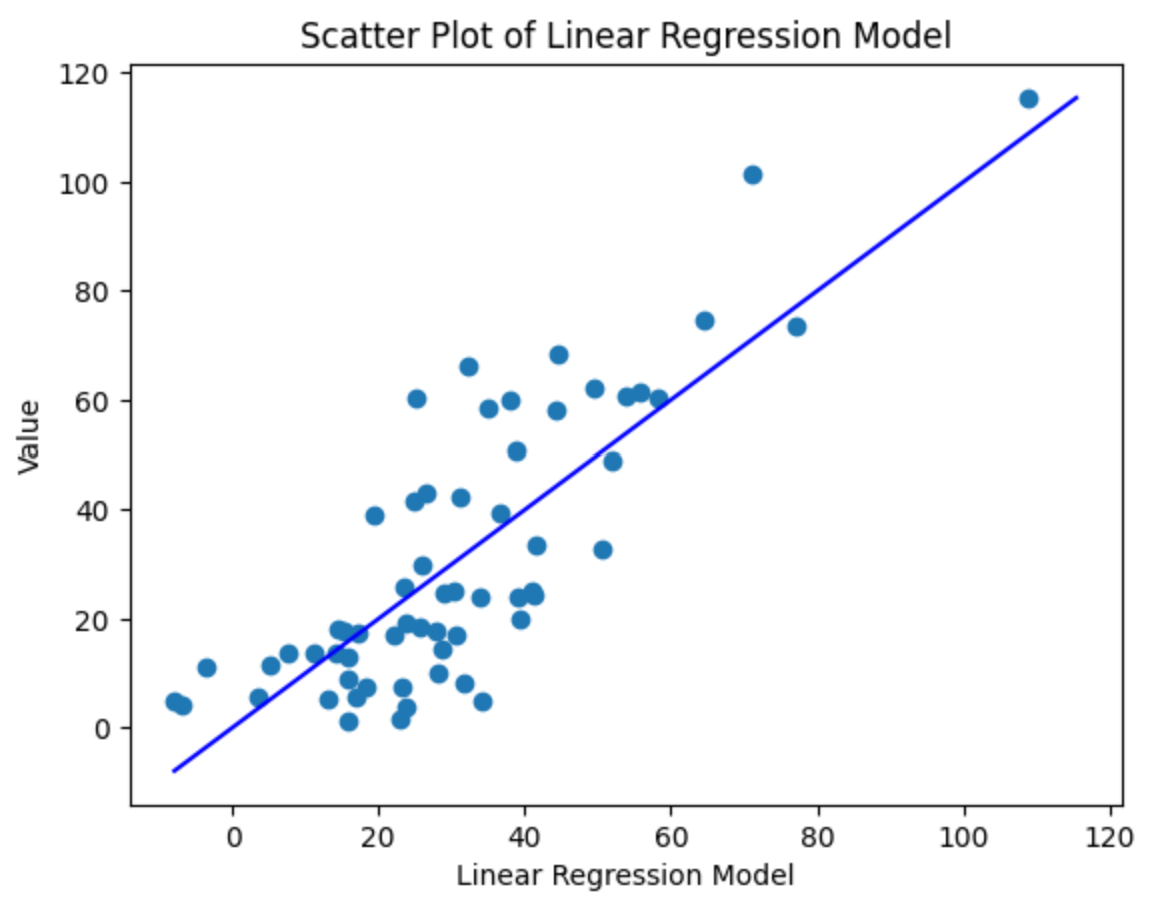
\includegraphics[width=6in,height=4.5in]{media/image5.png}
    \caption{Predictions vs actual values}
\end{figure}

\begin{figure}[H]
    \centering
    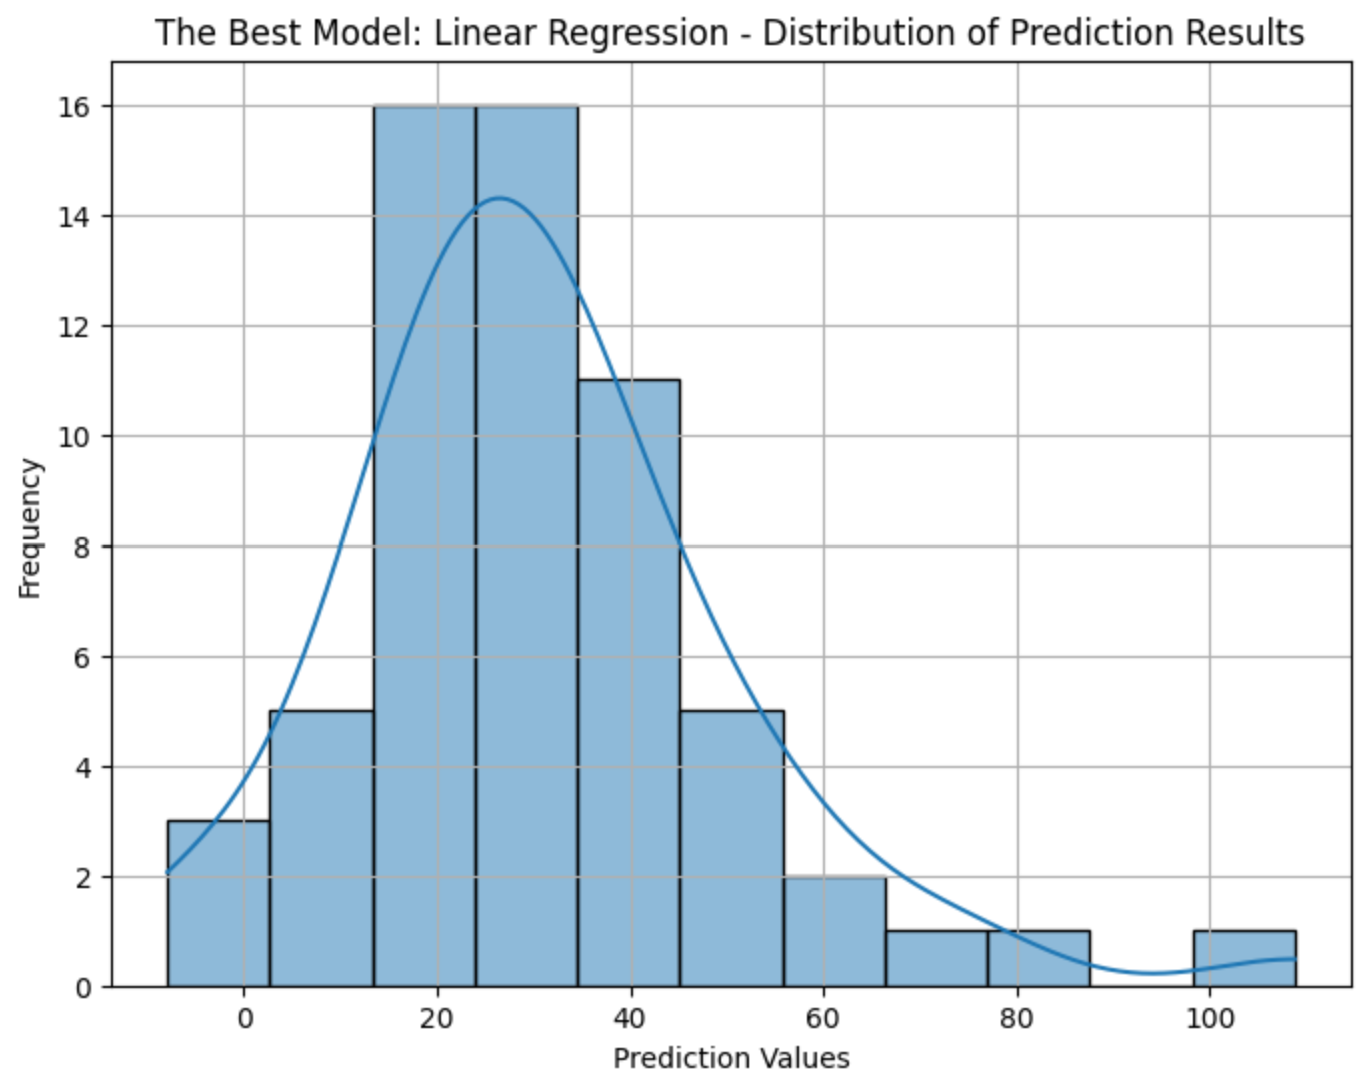
\includegraphics[width=6.5in,height=5in]{media/image1.png}
    \caption{Prediction distribution}
\end{figure}

% Thêm Conclusion như một phần riêng biệt
\cleardoublepage  % Start on a new right-hand page (nếu cần)
\phantomsection  % For hyperref compatibility
\addcontentsline{toc}{chapter}{Conclusion}  % Add to TOC as a chapter

\section*{Conclusion}  % Không đánh số cho phần này

\subsection*{Positive Aspects}
\begin{itemize}
    \item Successfully integrated end-to-end data science processes, including web scraping, preprocessing, statistical analysis, clustering, and predictive modeling.
    \item Identified top-performing teams (Liverpool) and players, providing valuable metrics for football analytics.
    \item Generated histograms, PCA plots, and heatmaps to intuitively communicate data trends and model performance.
    \item Achieved a competitive test R² score of 0.67 for transfer value prediction using Linear Regression.
\end{itemize}

\subsection*{Negative Aspects}
\begin{itemize}
    \item Reliance on specific websites (FBref, FootballTransfers) risks data accessibility issues if APIs or site structures change.
    \item Imputing missing values with zeros and simplifying age formats ("23-45" to 23.12) may introduce inaccuracies.
    \item Cross-validation revealed moderate consistency (mean CV R² = 0.50), indicating potential overfitting to the training set.
    \item Position-specific metrics (goalkeeping stats) had high missing rates, limiting their utility in analysis.
\end{itemize}

\subsection*{Future Developments}
\begin{itemize}
    \item Expand datasets to include multiple seasons or leagues (La Liga, Bundesliga) for broader insights.
    \item Experiment with ensemble methods (XGBoost, neural networks) to improve prediction accuracy and handle non-linear relationships.
    \item Develop automated pipelines to handle API changes and ensure long-term data accessibility.
\end{itemize}

\cleardoublepage  % Start on a new right-hand page (nếu cần)
\phantomsection  % For hyperref compatibility
\addcontentsline{toc}{chapter}{References}  % Add to TOC as a chapter
\chapter*{References}

\section*{Data Sources}  
    \textbf{FBref.com}: Football Statistics and Analysis. Retrieved from \href{https://fbref.com/}{https://fbref.com/}  

    \textbf{FootballTransfers.com}: Player Transfer Values and Market Insights. Retrieved from \href{https://www.footballtransfers.com/}{https://www.footballtransfers.com/}

\section*{Python Libraries \& Tools}  
    \textbf{pandas}: Powerful data manipulation and analysis toolkit. Retrieved from \href{https://pandas.pydata.org/}{https://pandas.pydata.org/}  

    \textbf{BeautifulSoup}: Library for parsing HTML and XML documents. Retrieved from \href{https://www.crummy.com/software/BeautifulSoup/}{https://www.crummy.com/software/BeautifulSoup/}  

    \textbf{scikit-learn}: Machine learning library for Python. Retrieved from \href{https://scikit-learn.org/}{https://scikit-learn.org/}  

    \textbf{matplotlib}: Comprehensive plotting library. Retrieved from \href{https://matplotlib.org/}{https://matplotlib.org/}  

    \textbf{seaborn}: Statistical data visualization library. Retrieved from \href{https://seaborn.pydata.org/}{https://seaborn.pydata.org/}  

    \textbf{requests}: HTTP library for Python. Retrieved from \href{https://requests.readthedocs.io/}{https://requests.readthedocs.io/}  

    \textbf{rapidfuzz}: Fast string matching library. Retrieved from \href{https://github.com/maxbachmann/RapidFuzz}{https://github.com/maxbachmann/RapidFuzz}  

    \textbf{unidecode}: Text normalization for Unicode characters. Retrieved from \href{https://pypi.org/project/Unidecode/}{https://pypi.org/project/Unidecode/}

\section*{Methodology \& Algorithms}  
    \textbf{K-means Clustering}: Unsupervised clustering algorithm. Scikit-learn Documentation. Retrieved from \href{https://scikit-learn.org/stable/modules/clustering.html\#k-means}{https://scikit-learn.org/stable/modules/clustering.html\#k-means}  

    \textbf{Principal Component Analysis (PCA)}: Dimensionality reduction technique. Scikit-learn Documentation. Retrieved from \href{https://scikit-learn.org/stable/modules/decomposition.html\#pca}{https://scikit-learn.org/stable/modules/decomposition.html\#pca}

\end{document}
